\documentclass[twoside]{book}

% Packages required by doxygen
\usepackage{fixltx2e}
\usepackage{calc}
\usepackage{doxygen}
\usepackage[export]{adjustbox} % also loads graphicx
\usepackage{graphicx}
\usepackage[utf8]{inputenc}
\usepackage{makeidx}
\usepackage{multicol}
\usepackage{multirow}
\PassOptionsToPackage{warn}{textcomp}
\usepackage{textcomp}
\usepackage[nointegrals]{wasysym}
\usepackage[table]{xcolor}

% Font selection
\usepackage[T1]{fontenc}
\usepackage[scaled=.90]{helvet}
\usepackage{courier}
\usepackage{amssymb}
\usepackage{sectsty}
\renewcommand{\familydefault}{\sfdefault}
\allsectionsfont{%
  \fontseries{bc}\selectfont%
  \color{darkgray}%
}
\renewcommand{\DoxyLabelFont}{%
  \fontseries{bc}\selectfont%
  \color{darkgray}%
}
\newcommand{\+}{\discretionary{\mbox{\scriptsize$\hookleftarrow$}}{}{}}

% Page & text layout
\usepackage{geometry}
\geometry{%
  a4paper,%
  top=2.5cm,%
  bottom=2.5cm,%
  left=2.5cm,%
  right=2.5cm%
}
\tolerance=750
\hfuzz=15pt
\hbadness=750
\setlength{\emergencystretch}{15pt}
\setlength{\parindent}{0cm}
\setlength{\parskip}{3ex plus 2ex minus 2ex}
\makeatletter
\renewcommand{\paragraph}{%
  \@startsection{paragraph}{4}{0ex}{-1.0ex}{1.0ex}{%
    \normalfont\normalsize\bfseries\SS@parafont%
  }%
}
\renewcommand{\subparagraph}{%
  \@startsection{subparagraph}{5}{0ex}{-1.0ex}{1.0ex}{%
    \normalfont\normalsize\bfseries\SS@subparafont%
  }%
}
\makeatother

% Headers & footers
\usepackage{fancyhdr}
\pagestyle{fancyplain}
\fancyhead[LE]{\fancyplain{}{\bfseries\thepage}}
\fancyhead[CE]{\fancyplain{}{}}
\fancyhead[RE]{\fancyplain{}{\bfseries\leftmark}}
\fancyhead[LO]{\fancyplain{}{\bfseries\rightmark}}
\fancyhead[CO]{\fancyplain{}{}}
\fancyhead[RO]{\fancyplain{}{\bfseries\thepage}}
\fancyfoot[LE]{\fancyplain{}{}}
\fancyfoot[CE]{\fancyplain{}{}}
\fancyfoot[RE]{\fancyplain{}{\bfseries\scriptsize Generated by Doxygen }}
\fancyfoot[LO]{\fancyplain{}{\bfseries\scriptsize Generated by Doxygen }}
\fancyfoot[CO]{\fancyplain{}{}}
\fancyfoot[RO]{\fancyplain{}{}}
\renewcommand{\footrulewidth}{0.4pt}
\renewcommand{\chaptermark}[1]{%
  \markboth{#1}{}%
}
\renewcommand{\sectionmark}[1]{%
  \markright{\thesection\ #1}%
}

% Indices & bibliography
\usepackage{natbib}
\usepackage[titles]{tocloft}
\setcounter{tocdepth}{3}
\setcounter{secnumdepth}{5}
\makeindex

% Hyperlinks (required, but should be loaded last)
\usepackage{ifpdf}
\ifpdf
  \usepackage[pdftex,pagebackref=true]{hyperref}
\else
  \usepackage[ps2pdf,pagebackref=true]{hyperref}
\fi
\hypersetup{%
  colorlinks=true,%
  linkcolor=blue,%
  citecolor=blue,%
  unicode%
}

% Custom commands
\newcommand{\clearemptydoublepage}{%
  \newpage{\pagestyle{empty}\cleardoublepage}%
}

\usepackage{caption}
\captionsetup{labelsep=space,justification=centering,font={bf},singlelinecheck=off,skip=4pt,position=top}

%===== C O N T E N T S =====

\begin{document}

% Titlepage & ToC
\hypersetup{pageanchor=false,
             bookmarksnumbered=true,
             pdfencoding=unicode
            }
\pagenumbering{alph}
\begin{titlepage}
\vspace*{7cm}
\begin{center}%
{\Large Reference Manual\\[1ex]\large v2.\+0 }\\
\vspace*{1cm}
{\large Generated by Doxygen 1.8.13}\\
\end{center}
\end{titlepage}
\clearemptydoublepage
\pagenumbering{roman}
\tableofcontents
\clearemptydoublepage
\pagenumbering{arabic}
\hypersetup{pageanchor=true}

%--- Begin generated contents ---
\chapter{R\+E\+A\+D\+ME}
\label{md__r_e_a_d_m_e}
\Hypertarget{md__r_e_a_d_m_e}


\href{https://travis-ci.org/RajPShinde/Autonomous_Wheelchair}{\tt } \href{https://coveralls.io/github/RajPShinde/Autonomous_Wheelchair?branch=master&service=github}{\tt } \href{https://github.com/RajPShinde/Autonomous_Wheelchair/blob/master/LICENSE}{\tt } \subsection*{\href{https://github.com/RajPShinde/Autonomous_Wheelchair/docs}{\tt } }

\subsection*{Authors}


\begin{DoxyItemize}
\item {\bfseries Raj Prakash Shinde} \href{https://github.com/RajPShinde}{\tt Git\+Hub} ~\newline
I am a Masters in Robotics Engineering student at the University of Maryland, College Park. My primary area of interest are Legged Robotics and Automation.
\item {\bfseries Shubham Sonawane} \href{https://github.com/shubham1925}{\tt Git\+Hub} ~\newline
I am a Master\textquotesingle{}s in Robotics Engineering student at the University of Maryland, College Park.
\item {\bfseries Prasheel Renkuntla} \href{https://github.com/Prasheel24}{\tt Git\+Hub} ~\newline
I am a Master\textquotesingle{}s in Robotics Engineering student at the University of Maryland, College Park. My primary area of interest is in Vision integrated Robot Systems.
\end{DoxyItemize}

\subsection*{Overview}

A R\+OS Stack to make a Wheelchair Navigate Wheelchair Autonomously in an indoor Environment.

\subsection*{Description}

\subsection*{Sprint Planning and Discussion}

Sprint Discussion\textquotesingle{}s -\/ \href{https://docs.google.com/document/d/1YxuiONLKsmspN5a6GJSREl9pPx3vZLULn2Mh-LnGHLA/edit?usp=sharing}{\tt Link}

\subsection*{Agile Iterative Process Log}

Access Product Backlog, Worklog \& Iteration Log here-\/ \href{https://docs.google.com/spreadsheets/d/16jTj_WTD0Le5l6ijkAiI3PhKVDuv9GQzufeO_Imgy9o/edit?usp=sharing}{\tt Link}

\subsection*{Dependencies}


\begin{DoxyEnumerate}
\item Ubuntu 16.\+04
\item C++ 11/14/17
\end{DoxyEnumerate}

\subsection*{Build}

Steps to build 
\begin{DoxyCode}
mkdir -p ~/catkin\_ws/src
cd ~/catkin\_ws/
catkin\_make
source devel/setup.bash
cd src/
git clone https://github.com/RajPShinde/Autonomous\_Wheelchair
cd ~/catkin\_ws/
catkin\_make
\end{DoxyCode}


\subsection*{Disclaimer}


\begin{DoxyCode}
BSD 3-Clause License

Copyright (c) 2020, Raj Shinde
Copyright (c) 2020, Prasheel Renkuntla
Copyright (c) 2020, Shubham Sonawane
All rights reserved.

Redistribution and use in source and binary forms, with or without
modification, are permitted provided that the following conditions are met:

1. Redistributions of source code must retain the above copyright notice, this
   list of conditions and the following disclaimer.

2. Redistributions in binary form must reproduce the above copyright notice,
   this list of conditions and the following disclaimer in the documentation
   and/or other materials provided with the distribution.

3. Neither the name of the copyright holder nor the names of its
   contributors may be used to endorse or promote products derived from
   this software without specific prior written permission.

THIS SOFTWARE IS PROVIDED BY THE COPYRIGHT HOLDERS AND CONTRIBUTORS "AS IS"
AND ANY EXPRESS OR IMPLIED WARRANTIES, INCLUDING, BUT NOT LIMITED TO, THE
IMPLIED WARRANTIES OF MERCHANTABILITY AND FITNESS FOR A PARTICULAR PURPOSE ARE
DISCLAIMED. IN NO EVENT SHALL THE COPYRIGHT HOLDER OR CONTRIBUTORS BE LIABLE
FOR ANY DIRECT, INDIRECT, INCIDENTAL, SPECIAL, EXEMPLARY, OR CONSEQUENTIAL
DAMAGES (INCLUDING, BUT NOT LIMITED TO, PROCUREMENT OF SUBSTITUTE GOODS OR
SERVICES; LOSS OF USE, DATA, OR PROFITS; OR BUSINESS INTERRUPTION) HOWEVER
CAUSED AND ON ANY THEORY OF LIABILITY, WHETHER IN CONTRACT, STRICT LIABILITY,
OR TORT (INCLUDING NEGLIGENCE OR OTHERWISE) ARISING IN ANY WAY OUT OF THE USE
OF THIS SOFTWARE, EVEN IF ADVISED OF THE POSSIBILITY OF SUCH DAMAGE.
\end{DoxyCode}
 
\chapter{Hierarchical Index}
\section{Class Hierarchy}
This inheritance list is sorted roughly, but not completely, alphabetically\+:\begin{DoxyCompactList}
\item Base\+Global\+Planner\begin{DoxyCompactList}
\item \contentsline{section}{astar\+\_\+plugin\+:\+:A\+Star\+Planner}{\pageref{classastar__plugin_1_1_a_star_planner}}{}
\end{DoxyCompactList}
\item \contentsline{section}{Goal}{\pageref{class_goal}}{}
\item \contentsline{section}{Grid\+Square}{\pageref{class_grid_square}}{}
\item \contentsline{section}{Navigate\+Robot}{\pageref{class_navigate_robot}}{}
\end{DoxyCompactList}

\chapter{Class Index}
\section{Class List}
Here are the classes, structs, unions and interfaces with brief descriptions\+:\begin{DoxyCompactList}
\item\contentsline{section}{\hyperlink{classastar__plugin_1_1_a_star_planner}{astar\+\_\+plugin\+::\+A\+Star\+Planner} }{\pageref{classastar__plugin_1_1_a_star_planner}}{}
\item\contentsline{section}{\hyperlink{class_goal}{Goal} }{\pageref{class_goal}}{}
\item\contentsline{section}{\hyperlink{class_grid_square}{Grid\+Square} }{\pageref{class_grid_square}}{}
\item\contentsline{section}{\hyperlink{class_navigate_robot}{Navigate\+Robot} }{\pageref{class_navigate_robot}}{}
\end{DoxyCompactList}

\chapter{File Index}
\section{File List}
Here is a list of all documented files with brief descriptions\+:\begin{DoxyCompactList}
\item\contentsline{section}{include/\hyperlink{goal_8hpp}{goal.\+hpp} \\*Autonomous Wheelchair }{\pageref{goal_8hpp}}{}
\item\contentsline{section}{include/{\bfseries grid\+Square.\+hpp} }{\pageref{grid_square_8hpp}}{}
\item\contentsline{section}{include/{\bfseries navigate\+Robot.\+hpp} }{\pageref{navigate_robot_8hpp}}{}
\item\contentsline{section}{include/{\bfseries path\+Planner.\+hpp} }{\pageref{path_planner_8hpp}}{}
\item\contentsline{section}{src/\hyperlink{goal_8cpp}{goal.\+cpp} \\*Autonomous Wheelchair }{\pageref{goal_8cpp}}{}
\item\contentsline{section}{src/\hyperlink{navigate_robot_8cpp}{navigate\+Robot.\+cpp} \\*Autonomous Wheelchair }{\pageref{navigate_robot_8cpp}}{}
\item\contentsline{section}{src/\hyperlink{path_planner_8cpp}{path\+Planner.\+cpp} \\*Autonomous wheelchair }{\pageref{path_planner_8cpp}}{}
\item\contentsline{section}{test/\hyperlink{test_grid_square_8cpp}{test\+Grid\+Square.\+cpp} \\*Autonomous Wheelchair }{\pageref{test_grid_square_8cpp}}{}
\item\contentsline{section}{test/\hyperlink{test_navigate_robot_8cpp}{test\+Navigate\+Robot.\+cpp} \\*Autonomous Wheelchair }{\pageref{test_navigate_robot_8cpp}}{}
\end{DoxyCompactList}

\chapter{Class Documentation}
\hypertarget{classastar__plugin_1_1_a_star_planner}{}\section{astar\+\_\+plugin\+:\+:A\+Star\+Planner Class Reference}
\label{classastar__plugin_1_1_a_star_planner}\index{astar\+\_\+plugin\+::\+A\+Star\+Planner@{astar\+\_\+plugin\+::\+A\+Star\+Planner}}


Inheritance diagram for astar\+\_\+plugin\+:\+:A\+Star\+Planner\+:
\nopagebreak
\begin{figure}[H]
\begin{center}
\leavevmode
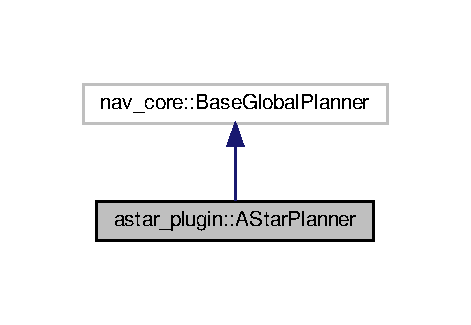
\includegraphics[width=226pt]{classastar__plugin_1_1_a_star_planner__inherit__graph}
\end{center}
\end{figure}


Collaboration diagram for astar\+\_\+plugin\+:\+:A\+Star\+Planner\+:
\nopagebreak
\begin{figure}[H]
\begin{center}
\leavevmode
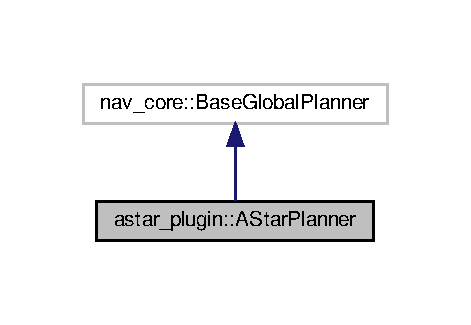
\includegraphics[width=226pt]{classastar__plugin_1_1_a_star_planner__coll__graph}
\end{center}
\end{figure}
\subsection*{Public Member Functions}
\begin{DoxyCompactItemize}
\item 
\hyperlink{classastar__plugin_1_1_a_star_planner_a709090708527da7d103f7c9373f4b651}{A\+Star\+Planner} ()
\begin{DoxyCompactList}\small\item\em Constructor of class A\+Star planner. \end{DoxyCompactList}\item 
\hyperlink{classastar__plugin_1_1_a_star_planner_a79cd3d4231e807ccc04f70d1e4ecd837}{A\+Star\+Planner} (ros\+::\+Node\+Handle \&)
\begin{DoxyCompactList}\small\item\em Overloaded constructor to call ros node handle. \end{DoxyCompactList}\item 
\hyperlink{classastar__plugin_1_1_a_star_planner_a6eaf79c8595c501e03117436fd499e42}{A\+Star\+Planner} (std\+::string name, costmap\+\_\+2d\+::\+Costmap2\+D\+R\+OS $\ast$costmap\+\_\+ros)
\begin{DoxyCompactList}\small\item\em Overloaded constructor to initialise 2D cost map. \end{DoxyCompactList}\item 
void \hyperlink{classastar__plugin_1_1_a_star_planner_abd555da48b7cb20f1fef16962ac0a71c}{initialize} (std\+::string name, costmap\+\_\+2d\+::\+Costmap2\+D\+R\+OS $\ast$costmap\+\_\+ros)
\begin{DoxyCompactList}\small\item\em Function inherited from base class to initialise map. \end{DoxyCompactList}\item 
bool \hyperlink{classastar__plugin_1_1_a_star_planner_a0452b64fca4b454fad7da2249494a9fd}{make\+Plan} (const geometry\+\_\+msgs\+::\+Pose\+Stamped \&start, const geometry\+\_\+msgs\+::\+Pose\+Stamped \&goal, std\+::vector$<$ geometry\+\_\+msgs\+::\+Pose\+Stamped $>$ \&plan)
\begin{DoxyCompactList}\small\item\em Function to make a plan to reach the goal. \end{DoxyCompactList}\item 
std\+::vector$<$ int $>$ \hyperlink{classastar__plugin_1_1_a_star_planner_a70e9cb8c51872dd8f83d1ae4a7006c62}{run\+A\+Star} (int start\+Cell, int goal\+Cell)
\begin{DoxyCompactList}\small\item\em Function to run astar algorithm. \end{DoxyCompactList}\item 
std\+::vector$<$ int $>$ \hyperlink{classastar__plugin_1_1_a_star_planner_a65c23083aa562f0ce8a881d26fb020a7}{find\+Path} (int start\+Cell, int goal\+Cell, std\+::vector$<$ float $>$ g\+\_\+score)
\begin{DoxyCompactList}\small\item\em Function to find path to reach the goal. \end{DoxyCompactList}\item 
std\+::vector$<$ int $>$ \hyperlink{classastar__plugin_1_1_a_star_planner_aae75ccdcf38f6cd848d024a8aebc0bc0}{construct\+Path} (int start\+Cell, int goal\+Cell, std\+::vector$<$ float $>$ g\+\_\+score)
\begin{DoxyCompactList}\small\item\em Function to construct a path to reach the goal. \end{DoxyCompactList}\item 
std\+::vector$<$ float $>$ \hyperlink{classastar__plugin_1_1_a_star_planner_a875990bd4b8b9ab17855ce54b4df4780}{get\+Map\+Coordinates} (float x, float y)
\begin{DoxyCompactList}\small\item\em Function to get map coordinates. \end{DoxyCompactList}\item 
float \hyperlink{classastar__plugin_1_1_a_star_planner_a18fac92699522fa76a2add6ea75fa6fc}{calculate\+H\+Cell\+Score} (int cell\+Index, int cell\+Square)
\begin{DoxyCompactList}\small\item\em Function to calculate H cell score. \end{DoxyCompactList}\item 
int \hyperlink{classastar__plugin_1_1_a_star_planner_aa54d997cd223de69fb7a37a79dc5cd1c}{calculate\+Cell\+Index} (int i, int j)
\begin{DoxyCompactList}\small\item\em Function to calculate cell index. \end{DoxyCompactList}\item 
int \hyperlink{classastar__plugin_1_1_a_star_planner_a660c014cd14a8de3080b138b44f5437e}{get\+Cell\+Row\+Index} (int index)
\begin{DoxyCompactList}\small\item\em Function to get Cell Row index. \end{DoxyCompactList}\item 
int \hyperlink{classastar__plugin_1_1_a_star_planner_a7242cadadc720feb8af97bc9f427f53c}{get\+Cell\+Col\+Index} (int index)
\begin{DoxyCompactList}\small\item\em Function to get Cell Column index. \end{DoxyCompactList}\item 
bool \hyperlink{classastar__plugin_1_1_a_star_planner_a29d81e8f4ac6191296d5c180be9ac8ae}{is\+Cell\+Free} (int cell\+Index)
\begin{DoxyCompactList}\small\item\em Function to check if the cell is free. \end{DoxyCompactList}\item 
bool \hyperlink{classastar__plugin_1_1_a_star_planner_ae8f5105e002f679874c3d55815fe30ad}{is\+Cell\+Free} (int i, int j)
\begin{DoxyCompactList}\small\item\em Overloaded function to check if cell is free. \end{DoxyCompactList}\item 
float \hyperlink{classastar__plugin_1_1_a_star_planner_ad07f32fd3a1e44ef3bb9bb1e59237023}{get\+Move\+To\+Cell\+Cost} (int cell\+Index1, int cell\+Index2)
\begin{DoxyCompactList}\small\item\em Function to get moving cost to a cell. \end{DoxyCompactList}\item 
float \hyperlink{classastar__plugin_1_1_a_star_planner_a2f19049be7428c445b7159cc111b4401}{get\+Move\+To\+Cell\+Cost} (int i1, int j1, int i2, int j2)
\begin{DoxyCompactList}\small\item\em Overloaded function to get moving cost to a cell. \end{DoxyCompactList}\item 
std\+::vector$<$ int $>$ \hyperlink{classastar__plugin_1_1_a_star_planner_a5ea485f93bfba47034d611b04eba2189}{find\+Free\+Neighbor\+Cell} (int cell\+Index)
\begin{DoxyCompactList}\small\item\em Function to find free neighbouring cell to traverse. \end{DoxyCompactList}\item 
void \hyperlink{classastar__plugin_1_1_a_star_planner_ac43f501b17770643240a6e36174a73b9}{convert\+To\+Map\+Coordinates} (float \&x, float \&y)
\begin{DoxyCompactList}\small\item\em Function to convert coordinates into a static map. \end{DoxyCompactList}\item 
int \hyperlink{classastar__plugin_1_1_a_star_planner_aae9903fa7f48e8e1ce45f4c772989e95}{get\+Cell\+Index} (float x, float y)
\begin{DoxyCompactList}\small\item\em Function to get cell index. \end{DoxyCompactList}\item 
void \hyperlink{classastar__plugin_1_1_a_star_planner_add9c03d5a079ad44e5f91ccc8344679d}{get\+Cell\+Coordinates} (int index, float \&x, float \&y)
\begin{DoxyCompactList}\small\item\em Function to get cell coordinates. \end{DoxyCompactList}\item 
bool \hyperlink{classastar__plugin_1_1_a_star_planner_a3e3717511d9000f1c55f3f57a58dfd0f}{is\+Coordinate\+In\+Bounds} (float x, float y)
\begin{DoxyCompactList}\small\item\em Function to check whether given coordinates are under boundary. \end{DoxyCompactList}\item 
void \hyperlink{classastar__plugin_1_1_a_star_planner_a2d44c51604b31cd5f7e8599520ae3645}{add\+Neighbor\+Cell\+To\+Open\+List} (std\+::set$<$ \hyperlink{class_grid_square}{Grid\+Square} $>$ \&O\+PL, int neighbor\+Cell, int goal\+Cell, std\+::vector$<$ float $>$ g\+\_\+score)
\begin{DoxyCompactList}\small\item\em Function to add nearest neighbor to open list of coordinates. \end{DoxyCompactList}\item 
bool \hyperlink{classastar__plugin_1_1_a_star_planner_a755e2c8b550458a1c4640a86fca1d993}{is\+Start\+And\+Goal\+Valid} (int start\+Cell, int goal\+Cell)
\begin{DoxyCompactList}\small\item\em Function to check if the start and end goal are valid. \end{DoxyCompactList}\end{DoxyCompactItemize}
\subsection*{Public Attributes}
\begin{DoxyCompactItemize}
\item 
\mbox{\Hypertarget{classastar__plugin_1_1_a_star_planner_afb117804426fe5f1a9a882a0da06047a}\label{classastar__plugin_1_1_a_star_planner_afb117804426fe5f1a9a882a0da06047a}} 
int {\bfseries value}
\item 
\mbox{\Hypertarget{classastar__plugin_1_1_a_star_planner_a5edf65eab6aa9be80520ebbcaa9e6704}\label{classastar__plugin_1_1_a_star_planner_a5edf65eab6aa9be80520ebbcaa9e6704}} 
int {\bfseries map\+Size}
\item 
\mbox{\Hypertarget{classastar__plugin_1_1_a_star_planner_a205a9cf7b62779627bf89c8b0d78f391}\label{classastar__plugin_1_1_a_star_planner_a205a9cf7b62779627bf89c8b0d78f391}} 
bool $\ast$ {\bfseries occupancy\+Grid\+Map}
\item 
\mbox{\Hypertarget{classastar__plugin_1_1_a_star_planner_a0d9b3ad5c3a83a96192609939af84c3d}\label{classastar__plugin_1_1_a_star_planner_a0d9b3ad5c3a83a96192609939af84c3d}} 
float {\bfseries infinity} = std\+::numeric\+\_\+limits$<$float$>$\+::infinity()
\item 
\mbox{\Hypertarget{classastar__plugin_1_1_a_star_planner_aae46db226358860bb296612e97a67617}\label{classastar__plugin_1_1_a_star_planner_aae46db226358860bb296612e97a67617}} 
float {\bfseries t\+Break}
\item 
\mbox{\Hypertarget{classastar__plugin_1_1_a_star_planner_ab20d703c7c32c96a523295cf07f8ef99}\label{classastar__plugin_1_1_a_star_planner_ab20d703c7c32c96a523295cf07f8ef99}} 
ros\+::\+Node\+Handle {\bfseries R\+O\+S\+Node\+Handle}
\item 
\mbox{\Hypertarget{classastar__plugin_1_1_a_star_planner_a9accb42a886464ae84db5259aad9c444}\label{classastar__plugin_1_1_a_star_planner_a9accb42a886464ae84db5259aad9c444}} 
float {\bfseries originX}
\item 
\mbox{\Hypertarget{classastar__plugin_1_1_a_star_planner_aa680b5cf31ff141738c409c4e86dbba6}\label{classastar__plugin_1_1_a_star_planner_aa680b5cf31ff141738c409c4e86dbba6}} 
float {\bfseries originY}
\item 
\mbox{\Hypertarget{classastar__plugin_1_1_a_star_planner_a698245ae6075cbbcb7d50d949025df95}\label{classastar__plugin_1_1_a_star_planner_a698245ae6075cbbcb7d50d949025df95}} 
float {\bfseries resolution}
\item 
\mbox{\Hypertarget{classastar__plugin_1_1_a_star_planner_a1be22c40d97241edb0a60b7bd3c332f3}\label{classastar__plugin_1_1_a_star_planner_a1be22c40d97241edb0a60b7bd3c332f3}} 
costmap\+\_\+2d\+::\+Costmap2\+D\+R\+OS $\ast$ {\bfseries costmap\+\_\+ros}
\item 
\mbox{\Hypertarget{classastar__plugin_1_1_a_star_planner_afeaa9448af26fc54e8adb0a906bd6324}\label{classastar__plugin_1_1_a_star_planner_afeaa9448af26fc54e8adb0a906bd6324}} 
costmap\+\_\+2d\+::\+Costmap2D $\ast$ {\bfseries costmap}
\item 
\mbox{\Hypertarget{classastar__plugin_1_1_a_star_planner_a3befa689d0be167cbde58b71c635f5ae}\label{classastar__plugin_1_1_a_star_planner_a3befa689d0be167cbde58b71c635f5ae}} 
bool {\bfseries initialized}
\item 
\mbox{\Hypertarget{classastar__plugin_1_1_a_star_planner_a712676c797f8a99a81b7aa48e02d227b}\label{classastar__plugin_1_1_a_star_planner_a712676c797f8a99a81b7aa48e02d227b}} 
int {\bfseries width}
\item 
\mbox{\Hypertarget{classastar__plugin_1_1_a_star_planner_ad3806c8e75f4008de6b4ba1a1cbd2c42}\label{classastar__plugin_1_1_a_star_planner_ad3806c8e75f4008de6b4ba1a1cbd2c42}} 
int {\bfseries height}
\end{DoxyCompactItemize}


\subsection{Constructor \& Destructor Documentation}
\mbox{\Hypertarget{classastar__plugin_1_1_a_star_planner_a709090708527da7d103f7c9373f4b651}\label{classastar__plugin_1_1_a_star_planner_a709090708527da7d103f7c9373f4b651}} 
\index{astar\+\_\+plugin\+::\+A\+Star\+Planner@{astar\+\_\+plugin\+::\+A\+Star\+Planner}!A\+Star\+Planner@{A\+Star\+Planner}}
\index{A\+Star\+Planner@{A\+Star\+Planner}!astar\+\_\+plugin\+::\+A\+Star\+Planner@{astar\+\_\+plugin\+::\+A\+Star\+Planner}}
\subsubsection{\texorpdfstring{A\+Star\+Planner()}{AStarPlanner()}\hspace{0.1cm}{\footnotesize\ttfamily [1/3]}}
{\footnotesize\ttfamily astar\+\_\+plugin\+::\+A\+Star\+Planner\+::\+A\+Star\+Planner (\begin{DoxyParamCaption}{ }\end{DoxyParamCaption})}



Constructor of class A\+Star planner. 


\begin{DoxyParams}{Parameters}
{\em none} & \\
\hline
\end{DoxyParams}
\begin{DoxyReturn}{Returns}
none 
\end{DoxyReturn}
\mbox{\Hypertarget{classastar__plugin_1_1_a_star_planner_a79cd3d4231e807ccc04f70d1e4ecd837}\label{classastar__plugin_1_1_a_star_planner_a79cd3d4231e807ccc04f70d1e4ecd837}} 
\index{astar\+\_\+plugin\+::\+A\+Star\+Planner@{astar\+\_\+plugin\+::\+A\+Star\+Planner}!A\+Star\+Planner@{A\+Star\+Planner}}
\index{A\+Star\+Planner@{A\+Star\+Planner}!astar\+\_\+plugin\+::\+A\+Star\+Planner@{astar\+\_\+plugin\+::\+A\+Star\+Planner}}
\subsubsection{\texorpdfstring{A\+Star\+Planner()}{AStarPlanner()}\hspace{0.1cm}{\footnotesize\ttfamily [2/3]}}
{\footnotesize\ttfamily astar\+\_\+plugin\+::\+A\+Star\+Planner\+::\+A\+Star\+Planner (\begin{DoxyParamCaption}\item[{ros\+::\+Node\+Handle \&}]{nh }\end{DoxyParamCaption})\hspace{0.3cm}{\ttfamily [explicit]}}



Overloaded constructor to call ros node handle. 


\begin{DoxyParams}{Parameters}
{\em ros\+::\+Node\+Handle} & \\
\hline
\end{DoxyParams}
\begin{DoxyReturn}{Returns}
none 
\end{DoxyReturn}
\mbox{\Hypertarget{classastar__plugin_1_1_a_star_planner_a6eaf79c8595c501e03117436fd499e42}\label{classastar__plugin_1_1_a_star_planner_a6eaf79c8595c501e03117436fd499e42}} 
\index{astar\+\_\+plugin\+::\+A\+Star\+Planner@{astar\+\_\+plugin\+::\+A\+Star\+Planner}!A\+Star\+Planner@{A\+Star\+Planner}}
\index{A\+Star\+Planner@{A\+Star\+Planner}!astar\+\_\+plugin\+::\+A\+Star\+Planner@{astar\+\_\+plugin\+::\+A\+Star\+Planner}}
\subsubsection{\texorpdfstring{A\+Star\+Planner()}{AStarPlanner()}\hspace{0.1cm}{\footnotesize\ttfamily [3/3]}}
{\footnotesize\ttfamily astar\+\_\+plugin\+::\+A\+Star\+Planner\+::\+A\+Star\+Planner (\begin{DoxyParamCaption}\item[{std\+::string}]{name,  }\item[{costmap\+\_\+2d\+::\+Costmap2\+D\+R\+OS $\ast$}]{costmap\+\_\+ros }\end{DoxyParamCaption})}



Overloaded constructor to initialise 2D cost map. 


\begin{DoxyParams}{Parameters}
{\em string,name} & \\
\hline
{\em costmap\+\_\+2d\+::\+Costmap2\+D\+R\+OS,R\+OS} & 2D cost map \\
\hline
\end{DoxyParams}
\begin{DoxyReturn}{Returns}
none 
\end{DoxyReturn}


\subsection{Member Function Documentation}
\mbox{\Hypertarget{classastar__plugin_1_1_a_star_planner_a2d44c51604b31cd5f7e8599520ae3645}\label{classastar__plugin_1_1_a_star_planner_a2d44c51604b31cd5f7e8599520ae3645}} 
\index{astar\+\_\+plugin\+::\+A\+Star\+Planner@{astar\+\_\+plugin\+::\+A\+Star\+Planner}!add\+Neighbor\+Cell\+To\+Open\+List@{add\+Neighbor\+Cell\+To\+Open\+List}}
\index{add\+Neighbor\+Cell\+To\+Open\+List@{add\+Neighbor\+Cell\+To\+Open\+List}!astar\+\_\+plugin\+::\+A\+Star\+Planner@{astar\+\_\+plugin\+::\+A\+Star\+Planner}}
\subsubsection{\texorpdfstring{add\+Neighbor\+Cell\+To\+Open\+List()}{addNeighborCellToOpenList()}}
{\footnotesize\ttfamily void astar\+\_\+plugin\+::\+A\+Star\+Planner\+::add\+Neighbor\+Cell\+To\+Open\+List (\begin{DoxyParamCaption}\item[{std\+::set$<$ \hyperlink{class_grid_square}{Grid\+Square} $>$ \&}]{O\+PL,  }\item[{int}]{neighbor\+Cell,  }\item[{int}]{goal\+Cell,  }\item[{std\+::vector$<$ float $>$}]{g\+\_\+score }\end{DoxyParamCaption})}



Function to add nearest neighbor to open list of coordinates. 


\begin{DoxyParams}{Parameters}
{\em std\+::set$<$\+Grid\+Square$>$,set} & of coordinates \\
\hline
{\em int,neighbour} & cell \\
\hline
{\em int,goal} & cell \\
\hline
{\em std\+::vector$<$float$>$,current} & g function value for cell \\
\hline
\end{DoxyParams}
\begin{DoxyReturn}{Returns}
none 
\end{DoxyReturn}
\mbox{\Hypertarget{classastar__plugin_1_1_a_star_planner_aa54d997cd223de69fb7a37a79dc5cd1c}\label{classastar__plugin_1_1_a_star_planner_aa54d997cd223de69fb7a37a79dc5cd1c}} 
\index{astar\+\_\+plugin\+::\+A\+Star\+Planner@{astar\+\_\+plugin\+::\+A\+Star\+Planner}!calculate\+Cell\+Index@{calculate\+Cell\+Index}}
\index{calculate\+Cell\+Index@{calculate\+Cell\+Index}!astar\+\_\+plugin\+::\+A\+Star\+Planner@{astar\+\_\+plugin\+::\+A\+Star\+Planner}}
\subsubsection{\texorpdfstring{calculate\+Cell\+Index()}{calculateCellIndex()}}
{\footnotesize\ttfamily int astar\+\_\+plugin\+::\+A\+Star\+Planner\+::calculate\+Cell\+Index (\begin{DoxyParamCaption}\item[{int}]{i,  }\item[{int}]{j }\end{DoxyParamCaption})}



Function to calculate cell index. 


\begin{DoxyParams}{Parameters}
{\em int,cell} & y value \\
\hline
{\em int,cell} & x value \\
\hline
\end{DoxyParams}
\begin{DoxyReturn}{Returns}
int, cell index 
\end{DoxyReturn}
\mbox{\Hypertarget{classastar__plugin_1_1_a_star_planner_a18fac92699522fa76a2add6ea75fa6fc}\label{classastar__plugin_1_1_a_star_planner_a18fac92699522fa76a2add6ea75fa6fc}} 
\index{astar\+\_\+plugin\+::\+A\+Star\+Planner@{astar\+\_\+plugin\+::\+A\+Star\+Planner}!calculate\+H\+Cell\+Score@{calculate\+H\+Cell\+Score}}
\index{calculate\+H\+Cell\+Score@{calculate\+H\+Cell\+Score}!astar\+\_\+plugin\+::\+A\+Star\+Planner@{astar\+\_\+plugin\+::\+A\+Star\+Planner}}
\subsubsection{\texorpdfstring{calculate\+H\+Cell\+Score()}{calculateHCellScore()}}
{\footnotesize\ttfamily float astar\+\_\+plugin\+::\+A\+Star\+Planner\+::calculate\+H\+Cell\+Score (\begin{DoxyParamCaption}\item[{int}]{cell\+Index,  }\item[{int}]{cell\+Square }\end{DoxyParamCaption})}



Function to calculate H cell score. 


\begin{DoxyParams}{Parameters}
{\em int,cell} & index value \\
\hline
{\em int,cell} & limits \\
\hline
\end{DoxyParams}
\begin{DoxyReturn}{Returns}
float, H value 
\end{DoxyReturn}
\mbox{\Hypertarget{classastar__plugin_1_1_a_star_planner_aae75ccdcf38f6cd848d024a8aebc0bc0}\label{classastar__plugin_1_1_a_star_planner_aae75ccdcf38f6cd848d024a8aebc0bc0}} 
\index{astar\+\_\+plugin\+::\+A\+Star\+Planner@{astar\+\_\+plugin\+::\+A\+Star\+Planner}!construct\+Path@{construct\+Path}}
\index{construct\+Path@{construct\+Path}!astar\+\_\+plugin\+::\+A\+Star\+Planner@{astar\+\_\+plugin\+::\+A\+Star\+Planner}}
\subsubsection{\texorpdfstring{construct\+Path()}{constructPath()}}
{\footnotesize\ttfamily std\+::vector$<$ int $>$ astar\+\_\+plugin\+::\+A\+Star\+Planner\+::construct\+Path (\begin{DoxyParamCaption}\item[{int}]{start\+Cell,  }\item[{int}]{goal\+Cell,  }\item[{std\+::vector$<$ float $>$}]{g\+\_\+score }\end{DoxyParamCaption})}



Function to construct a path to reach the goal. 


\begin{DoxyParams}{Parameters}
{\em int,start} & cell \\
\hline
{\em int,goal} & cell \\
\hline
{\em std\+::vector$<$float$>$,g} & function value for each cell \\
\hline
\end{DoxyParams}
\begin{DoxyReturn}{Returns}
std\+::vector$<$int$>$, if correct, then best path else empty path 
\end{DoxyReturn}
\mbox{\Hypertarget{classastar__plugin_1_1_a_star_planner_ac43f501b17770643240a6e36174a73b9}\label{classastar__plugin_1_1_a_star_planner_ac43f501b17770643240a6e36174a73b9}} 
\index{astar\+\_\+plugin\+::\+A\+Star\+Planner@{astar\+\_\+plugin\+::\+A\+Star\+Planner}!convert\+To\+Map\+Coordinates@{convert\+To\+Map\+Coordinates}}
\index{convert\+To\+Map\+Coordinates@{convert\+To\+Map\+Coordinates}!astar\+\_\+plugin\+::\+A\+Star\+Planner@{astar\+\_\+plugin\+::\+A\+Star\+Planner}}
\subsubsection{\texorpdfstring{convert\+To\+Map\+Coordinates()}{convertToMapCoordinates()}}
{\footnotesize\ttfamily void astar\+\_\+plugin\+::\+A\+Star\+Planner\+::convert\+To\+Map\+Coordinates (\begin{DoxyParamCaption}\item[{float \&}]{x,  }\item[{float \&}]{y }\end{DoxyParamCaption})}



Function to convert coordinates into a static map. 


\begin{DoxyParams}{Parameters}
{\em int,x} & coordinate \\
\hline
{\em int,y} & coordinate \\
\hline
\end{DoxyParams}
\begin{DoxyReturn}{Returns}
none 
\end{DoxyReturn}
\mbox{\Hypertarget{classastar__plugin_1_1_a_star_planner_a5ea485f93bfba47034d611b04eba2189}\label{classastar__plugin_1_1_a_star_planner_a5ea485f93bfba47034d611b04eba2189}} 
\index{astar\+\_\+plugin\+::\+A\+Star\+Planner@{astar\+\_\+plugin\+::\+A\+Star\+Planner}!find\+Free\+Neighbor\+Cell@{find\+Free\+Neighbor\+Cell}}
\index{find\+Free\+Neighbor\+Cell@{find\+Free\+Neighbor\+Cell}!astar\+\_\+plugin\+::\+A\+Star\+Planner@{astar\+\_\+plugin\+::\+A\+Star\+Planner}}
\subsubsection{\texorpdfstring{find\+Free\+Neighbor\+Cell()}{findFreeNeighborCell()}}
{\footnotesize\ttfamily std\+::vector$<$ int $>$ astar\+\_\+plugin\+::\+A\+Star\+Planner\+::find\+Free\+Neighbor\+Cell (\begin{DoxyParamCaption}\item[{int}]{cell\+Index }\end{DoxyParamCaption})}



Function to find free neighbouring cell to traverse. 


\begin{DoxyParams}{Parameters}
{\em int,previous} & cell index \\
\hline
\end{DoxyParams}
\begin{DoxyReturn}{Returns}
std\+::vector$<$int$>$, new cell indices 
\end{DoxyReturn}
\mbox{\Hypertarget{classastar__plugin_1_1_a_star_planner_a65c23083aa562f0ce8a881d26fb020a7}\label{classastar__plugin_1_1_a_star_planner_a65c23083aa562f0ce8a881d26fb020a7}} 
\index{astar\+\_\+plugin\+::\+A\+Star\+Planner@{astar\+\_\+plugin\+::\+A\+Star\+Planner}!find\+Path@{find\+Path}}
\index{find\+Path@{find\+Path}!astar\+\_\+plugin\+::\+A\+Star\+Planner@{astar\+\_\+plugin\+::\+A\+Star\+Planner}}
\subsubsection{\texorpdfstring{find\+Path()}{findPath()}}
{\footnotesize\ttfamily std\+::vector$<$ int $>$ astar\+\_\+plugin\+::\+A\+Star\+Planner\+::find\+Path (\begin{DoxyParamCaption}\item[{int}]{start\+Cell,  }\item[{int}]{goal\+Cell,  }\item[{std\+::vector$<$ float $>$}]{g\+\_\+score }\end{DoxyParamCaption})}



Function to find path to reach the goal. 


\begin{DoxyParams}{Parameters}
{\em int,start} & cell \\
\hline
{\em int,goal} & cell \\
\hline
{\em std\+::vector$<$float$>$,g} & function value for each cell \\
\hline
\end{DoxyParams}
\begin{DoxyReturn}{Returns}
std\+::vector$<$int$>$, if correct, then best path else empty path 
\end{DoxyReturn}
\mbox{\Hypertarget{classastar__plugin_1_1_a_star_planner_a7242cadadc720feb8af97bc9f427f53c}\label{classastar__plugin_1_1_a_star_planner_a7242cadadc720feb8af97bc9f427f53c}} 
\index{astar\+\_\+plugin\+::\+A\+Star\+Planner@{astar\+\_\+plugin\+::\+A\+Star\+Planner}!get\+Cell\+Col\+Index@{get\+Cell\+Col\+Index}}
\index{get\+Cell\+Col\+Index@{get\+Cell\+Col\+Index}!astar\+\_\+plugin\+::\+A\+Star\+Planner@{astar\+\_\+plugin\+::\+A\+Star\+Planner}}
\subsubsection{\texorpdfstring{get\+Cell\+Col\+Index()}{getCellColIndex()}}
{\footnotesize\ttfamily int astar\+\_\+plugin\+::\+A\+Star\+Planner\+::get\+Cell\+Col\+Index (\begin{DoxyParamCaption}\item[{int}]{index }\end{DoxyParamCaption})}



Function to get Cell Column index. 


\begin{DoxyParams}{Parameters}
{\em int,cell} & index value \\
\hline
\end{DoxyParams}
\begin{DoxyReturn}{Returns}
int, cell column index 
\end{DoxyReturn}
\mbox{\Hypertarget{classastar__plugin_1_1_a_star_planner_add9c03d5a079ad44e5f91ccc8344679d}\label{classastar__plugin_1_1_a_star_planner_add9c03d5a079ad44e5f91ccc8344679d}} 
\index{astar\+\_\+plugin\+::\+A\+Star\+Planner@{astar\+\_\+plugin\+::\+A\+Star\+Planner}!get\+Cell\+Coordinates@{get\+Cell\+Coordinates}}
\index{get\+Cell\+Coordinates@{get\+Cell\+Coordinates}!astar\+\_\+plugin\+::\+A\+Star\+Planner@{astar\+\_\+plugin\+::\+A\+Star\+Planner}}
\subsubsection{\texorpdfstring{get\+Cell\+Coordinates()}{getCellCoordinates()}}
{\footnotesize\ttfamily void astar\+\_\+plugin\+::\+A\+Star\+Planner\+::get\+Cell\+Coordinates (\begin{DoxyParamCaption}\item[{int}]{index,  }\item[{float \&}]{x,  }\item[{float \&}]{y }\end{DoxyParamCaption})}



Function to get cell coordinates. 


\begin{DoxyParams}{Parameters}
{\em int,index} & \\
\hline
{\em float,x} & coordinate \\
\hline
{\em float,y} & coordinate \\
\hline
\end{DoxyParams}
\begin{DoxyReturn}{Returns}
none 
\end{DoxyReturn}
\mbox{\Hypertarget{classastar__plugin_1_1_a_star_planner_aae9903fa7f48e8e1ce45f4c772989e95}\label{classastar__plugin_1_1_a_star_planner_aae9903fa7f48e8e1ce45f4c772989e95}} 
\index{astar\+\_\+plugin\+::\+A\+Star\+Planner@{astar\+\_\+plugin\+::\+A\+Star\+Planner}!get\+Cell\+Index@{get\+Cell\+Index}}
\index{get\+Cell\+Index@{get\+Cell\+Index}!astar\+\_\+plugin\+::\+A\+Star\+Planner@{astar\+\_\+plugin\+::\+A\+Star\+Planner}}
\subsubsection{\texorpdfstring{get\+Cell\+Index()}{getCellIndex()}}
{\footnotesize\ttfamily int astar\+\_\+plugin\+::\+A\+Star\+Planner\+::get\+Cell\+Index (\begin{DoxyParamCaption}\item[{float}]{x,  }\item[{float}]{y }\end{DoxyParamCaption})}



Function to get cell index. 


\begin{DoxyParams}{Parameters}
{\em int,x} & coordinate \\
\hline
{\em int,y} & coordinate \\
\hline
\end{DoxyParams}
\begin{DoxyReturn}{Returns}
int, index of cell 
\end{DoxyReturn}
\mbox{\Hypertarget{classastar__plugin_1_1_a_star_planner_a660c014cd14a8de3080b138b44f5437e}\label{classastar__plugin_1_1_a_star_planner_a660c014cd14a8de3080b138b44f5437e}} 
\index{astar\+\_\+plugin\+::\+A\+Star\+Planner@{astar\+\_\+plugin\+::\+A\+Star\+Planner}!get\+Cell\+Row\+Index@{get\+Cell\+Row\+Index}}
\index{get\+Cell\+Row\+Index@{get\+Cell\+Row\+Index}!astar\+\_\+plugin\+::\+A\+Star\+Planner@{astar\+\_\+plugin\+::\+A\+Star\+Planner}}
\subsubsection{\texorpdfstring{get\+Cell\+Row\+Index()}{getCellRowIndex()}}
{\footnotesize\ttfamily int astar\+\_\+plugin\+::\+A\+Star\+Planner\+::get\+Cell\+Row\+Index (\begin{DoxyParamCaption}\item[{int}]{index }\end{DoxyParamCaption})}



Function to get Cell Row index. 


\begin{DoxyParams}{Parameters}
{\em int,cell} & index value \\
\hline
\end{DoxyParams}
\begin{DoxyReturn}{Returns}
int, cell row index 
\end{DoxyReturn}
\mbox{\Hypertarget{classastar__plugin_1_1_a_star_planner_a875990bd4b8b9ab17855ce54b4df4780}\label{classastar__plugin_1_1_a_star_planner_a875990bd4b8b9ab17855ce54b4df4780}} 
\index{astar\+\_\+plugin\+::\+A\+Star\+Planner@{astar\+\_\+plugin\+::\+A\+Star\+Planner}!get\+Map\+Coordinates@{get\+Map\+Coordinates}}
\index{get\+Map\+Coordinates@{get\+Map\+Coordinates}!astar\+\_\+plugin\+::\+A\+Star\+Planner@{astar\+\_\+plugin\+::\+A\+Star\+Planner}}
\subsubsection{\texorpdfstring{get\+Map\+Coordinates()}{getMapCoordinates()}}
{\footnotesize\ttfamily std\+::vector$<$ float $>$ astar\+\_\+plugin\+::\+A\+Star\+Planner\+::get\+Map\+Coordinates (\begin{DoxyParamCaption}\item[{float}]{x,  }\item[{float}]{y }\end{DoxyParamCaption})}



Function to get map coordinates. 


\begin{DoxyParams}{Parameters}
{\em float,x} & coordinate \\
\hline
{\em float,y} & coordinate \\
\hline
\end{DoxyParams}
\begin{DoxyReturn}{Returns}
std\+::vector$<$float$>$ returns map coordinates 
\end{DoxyReturn}
\mbox{\Hypertarget{classastar__plugin_1_1_a_star_planner_ad07f32fd3a1e44ef3bb9bb1e59237023}\label{classastar__plugin_1_1_a_star_planner_ad07f32fd3a1e44ef3bb9bb1e59237023}} 
\index{astar\+\_\+plugin\+::\+A\+Star\+Planner@{astar\+\_\+plugin\+::\+A\+Star\+Planner}!get\+Move\+To\+Cell\+Cost@{get\+Move\+To\+Cell\+Cost}}
\index{get\+Move\+To\+Cell\+Cost@{get\+Move\+To\+Cell\+Cost}!astar\+\_\+plugin\+::\+A\+Star\+Planner@{astar\+\_\+plugin\+::\+A\+Star\+Planner}}
\subsubsection{\texorpdfstring{get\+Move\+To\+Cell\+Cost()}{getMoveToCellCost()}\hspace{0.1cm}{\footnotesize\ttfamily [1/2]}}
{\footnotesize\ttfamily float astar\+\_\+plugin\+::\+A\+Star\+Planner\+::get\+Move\+To\+Cell\+Cost (\begin{DoxyParamCaption}\item[{int}]{cell\+Index1,  }\item[{int}]{cell\+Index2 }\end{DoxyParamCaption})}



Function to get moving cost to a cell. 


\begin{DoxyParams}{Parameters}
{\em int,first} & cell index \\
\hline
{\em int,second} & cell index \\
\hline
\end{DoxyParams}
\begin{DoxyReturn}{Returns}
float, cell cost 
\end{DoxyReturn}
\mbox{\Hypertarget{classastar__plugin_1_1_a_star_planner_a2f19049be7428c445b7159cc111b4401}\label{classastar__plugin_1_1_a_star_planner_a2f19049be7428c445b7159cc111b4401}} 
\index{astar\+\_\+plugin\+::\+A\+Star\+Planner@{astar\+\_\+plugin\+::\+A\+Star\+Planner}!get\+Move\+To\+Cell\+Cost@{get\+Move\+To\+Cell\+Cost}}
\index{get\+Move\+To\+Cell\+Cost@{get\+Move\+To\+Cell\+Cost}!astar\+\_\+plugin\+::\+A\+Star\+Planner@{astar\+\_\+plugin\+::\+A\+Star\+Planner}}
\subsubsection{\texorpdfstring{get\+Move\+To\+Cell\+Cost()}{getMoveToCellCost()}\hspace{0.1cm}{\footnotesize\ttfamily [2/2]}}
{\footnotesize\ttfamily float astar\+\_\+plugin\+::\+A\+Star\+Planner\+::get\+Move\+To\+Cell\+Cost (\begin{DoxyParamCaption}\item[{int}]{i1,  }\item[{int}]{j1,  }\item[{int}]{i2,  }\item[{int}]{j2 }\end{DoxyParamCaption})}



Overloaded function to get moving cost to a cell. 


\begin{DoxyParams}{Parameters}
{\em int,first} & cell x index \\
\hline
{\em int,first} & cell y index \\
\hline
{\em int,second} & cell x index \\
\hline
{\em int,second} & cell y index \\
\hline
\end{DoxyParams}
\begin{DoxyReturn}{Returns}
float, cell cost 
\end{DoxyReturn}
\mbox{\Hypertarget{classastar__plugin_1_1_a_star_planner_abd555da48b7cb20f1fef16962ac0a71c}\label{classastar__plugin_1_1_a_star_planner_abd555da48b7cb20f1fef16962ac0a71c}} 
\index{astar\+\_\+plugin\+::\+A\+Star\+Planner@{astar\+\_\+plugin\+::\+A\+Star\+Planner}!initialize@{initialize}}
\index{initialize@{initialize}!astar\+\_\+plugin\+::\+A\+Star\+Planner@{astar\+\_\+plugin\+::\+A\+Star\+Planner}}
\subsubsection{\texorpdfstring{initialize()}{initialize()}}
{\footnotesize\ttfamily void astar\+\_\+plugin\+::\+A\+Star\+Planner\+::initialize (\begin{DoxyParamCaption}\item[{std\+::string}]{name,  }\item[{costmap\+\_\+2d\+::\+Costmap2\+D\+R\+OS $\ast$}]{costmap\+\_\+ros }\end{DoxyParamCaption})}



Function inherited from base class to initialise map. 


\begin{DoxyParams}{Parameters}
{\em string,name} & \\
\hline
{\em costmap\+\_\+2d\+::\+Costmap2\+D\+R\+OS,R\+OS} & 2D cost map \\
\hline
\end{DoxyParams}
\begin{DoxyReturn}{Returns}
none 
\end{DoxyReturn}
\mbox{\Hypertarget{classastar__plugin_1_1_a_star_planner_a29d81e8f4ac6191296d5c180be9ac8ae}\label{classastar__plugin_1_1_a_star_planner_a29d81e8f4ac6191296d5c180be9ac8ae}} 
\index{astar\+\_\+plugin\+::\+A\+Star\+Planner@{astar\+\_\+plugin\+::\+A\+Star\+Planner}!is\+Cell\+Free@{is\+Cell\+Free}}
\index{is\+Cell\+Free@{is\+Cell\+Free}!astar\+\_\+plugin\+::\+A\+Star\+Planner@{astar\+\_\+plugin\+::\+A\+Star\+Planner}}
\subsubsection{\texorpdfstring{is\+Cell\+Free()}{isCellFree()}\hspace{0.1cm}{\footnotesize\ttfamily [1/2]}}
{\footnotesize\ttfamily bool astar\+\_\+plugin\+::\+A\+Star\+Planner\+::is\+Cell\+Free (\begin{DoxyParamCaption}\item[{int}]{cell\+Index }\end{DoxyParamCaption})}



Function to check if the cell is free. 


\begin{DoxyParams}{Parameters}
{\em int,cell} & index value \\
\hline
\end{DoxyParams}
\begin{DoxyReturn}{Returns}
bool, returns true if free 
\end{DoxyReturn}
\mbox{\Hypertarget{classastar__plugin_1_1_a_star_planner_ae8f5105e002f679874c3d55815fe30ad}\label{classastar__plugin_1_1_a_star_planner_ae8f5105e002f679874c3d55815fe30ad}} 
\index{astar\+\_\+plugin\+::\+A\+Star\+Planner@{astar\+\_\+plugin\+::\+A\+Star\+Planner}!is\+Cell\+Free@{is\+Cell\+Free}}
\index{is\+Cell\+Free@{is\+Cell\+Free}!astar\+\_\+plugin\+::\+A\+Star\+Planner@{astar\+\_\+plugin\+::\+A\+Star\+Planner}}
\subsubsection{\texorpdfstring{is\+Cell\+Free()}{isCellFree()}\hspace{0.1cm}{\footnotesize\ttfamily [2/2]}}
{\footnotesize\ttfamily bool astar\+\_\+plugin\+::\+A\+Star\+Planner\+::is\+Cell\+Free (\begin{DoxyParamCaption}\item[{int}]{i,  }\item[{int}]{j }\end{DoxyParamCaption})}



Overloaded function to check if cell is free. 


\begin{DoxyParams}{Parameters}
{\em int,cell} & x value \\
\hline
{\em int,cell} & y value \\
\hline
\end{DoxyParams}
\begin{DoxyReturn}{Returns}
bool, returns true if free 
\end{DoxyReturn}
\mbox{\Hypertarget{classastar__plugin_1_1_a_star_planner_a3e3717511d9000f1c55f3f57a58dfd0f}\label{classastar__plugin_1_1_a_star_planner_a3e3717511d9000f1c55f3f57a58dfd0f}} 
\index{astar\+\_\+plugin\+::\+A\+Star\+Planner@{astar\+\_\+plugin\+::\+A\+Star\+Planner}!is\+Coordinate\+In\+Bounds@{is\+Coordinate\+In\+Bounds}}
\index{is\+Coordinate\+In\+Bounds@{is\+Coordinate\+In\+Bounds}!astar\+\_\+plugin\+::\+A\+Star\+Planner@{astar\+\_\+plugin\+::\+A\+Star\+Planner}}
\subsubsection{\texorpdfstring{is\+Coordinate\+In\+Bounds()}{isCoordinateInBounds()}}
{\footnotesize\ttfamily bool astar\+\_\+plugin\+::\+A\+Star\+Planner\+::is\+Coordinate\+In\+Bounds (\begin{DoxyParamCaption}\item[{float}]{x,  }\item[{float}]{y }\end{DoxyParamCaption})}



Function to check whether given coordinates are under boundary. 


\begin{DoxyParams}{Parameters}
{\em int,x} & coordinate \\
\hline
{\em int,y} & coordinate \\
\hline
\end{DoxyParams}
\begin{DoxyReturn}{Returns}
bool, returns true if inside boundary 
\end{DoxyReturn}
\mbox{\Hypertarget{classastar__plugin_1_1_a_star_planner_a755e2c8b550458a1c4640a86fca1d993}\label{classastar__plugin_1_1_a_star_planner_a755e2c8b550458a1c4640a86fca1d993}} 
\index{astar\+\_\+plugin\+::\+A\+Star\+Planner@{astar\+\_\+plugin\+::\+A\+Star\+Planner}!is\+Start\+And\+Goal\+Valid@{is\+Start\+And\+Goal\+Valid}}
\index{is\+Start\+And\+Goal\+Valid@{is\+Start\+And\+Goal\+Valid}!astar\+\_\+plugin\+::\+A\+Star\+Planner@{astar\+\_\+plugin\+::\+A\+Star\+Planner}}
\subsubsection{\texorpdfstring{is\+Start\+And\+Goal\+Valid()}{isStartAndGoalValid()}}
{\footnotesize\ttfamily bool astar\+\_\+plugin\+::\+A\+Star\+Planner\+::is\+Start\+And\+Goal\+Valid (\begin{DoxyParamCaption}\item[{int}]{start\+Cell,  }\item[{int}]{goal\+Cell }\end{DoxyParamCaption})}



Function to check if the start and end goal are valid. 


\begin{DoxyParams}{Parameters}
{\em int,start} & cell \\
\hline
{\em int,goal} & cell \\
\hline
\end{DoxyParams}
\begin{DoxyReturn}{Returns}
bool, returns true if valid. 
\end{DoxyReturn}
\mbox{\Hypertarget{classastar__plugin_1_1_a_star_planner_a0452b64fca4b454fad7da2249494a9fd}\label{classastar__plugin_1_1_a_star_planner_a0452b64fca4b454fad7da2249494a9fd}} 
\index{astar\+\_\+plugin\+::\+A\+Star\+Planner@{astar\+\_\+plugin\+::\+A\+Star\+Planner}!make\+Plan@{make\+Plan}}
\index{make\+Plan@{make\+Plan}!astar\+\_\+plugin\+::\+A\+Star\+Planner@{astar\+\_\+plugin\+::\+A\+Star\+Planner}}
\subsubsection{\texorpdfstring{make\+Plan()}{makePlan()}}
{\footnotesize\ttfamily bool astar\+\_\+plugin\+::\+A\+Star\+Planner\+::make\+Plan (\begin{DoxyParamCaption}\item[{const geometry\+\_\+msgs\+::\+Pose\+Stamped \&}]{start,  }\item[{const geometry\+\_\+msgs\+::\+Pose\+Stamped \&}]{goal,  }\item[{std\+::vector$<$ geometry\+\_\+msgs\+::\+Pose\+Stamped $>$ \&}]{plan }\end{DoxyParamCaption})}



Function to make a plan to reach the goal. 


\begin{DoxyParams}{Parameters}
{\em const} & geometry\+\_\+msgs\+::\+Pose\+Stamped, start pose \\
\hline
{\em const} & geometry\+\_\+msgs\+::\+Pose\+Stamped, goal pose \\
\hline
{\em std\+::vector$<$geometry\+\_\+msgs\+::\+Pose\+Stamped$>$,vector} & plan to reach \\
\hline
\end{DoxyParams}
\begin{DoxyReturn}{Returns}
bool, returns true if plan exists 
\end{DoxyReturn}
\mbox{\Hypertarget{classastar__plugin_1_1_a_star_planner_a70e9cb8c51872dd8f83d1ae4a7006c62}\label{classastar__plugin_1_1_a_star_planner_a70e9cb8c51872dd8f83d1ae4a7006c62}} 
\index{astar\+\_\+plugin\+::\+A\+Star\+Planner@{astar\+\_\+plugin\+::\+A\+Star\+Planner}!run\+A\+Star@{run\+A\+Star}}
\index{run\+A\+Star@{run\+A\+Star}!astar\+\_\+plugin\+::\+A\+Star\+Planner@{astar\+\_\+plugin\+::\+A\+Star\+Planner}}
\subsubsection{\texorpdfstring{run\+A\+Star()}{runAStar()}}
{\footnotesize\ttfamily std\+::vector$<$ int $>$ astar\+\_\+plugin\+::\+A\+Star\+Planner\+::run\+A\+Star (\begin{DoxyParamCaption}\item[{int}]{start\+Cell,  }\item[{int}]{goal\+Cell }\end{DoxyParamCaption})}



Function to run astar algorithm. 


\begin{DoxyParams}{Parameters}
{\em int,start} & cell \\
\hline
{\em int,goal} & cell \\
\hline
\end{DoxyParams}
\begin{DoxyReturn}{Returns}
std\+::vector$<$int$>$, returns best path coordinates 
\end{DoxyReturn}


The documentation for this class was generated from the following files\+:\begin{DoxyCompactItemize}
\item 
include/path\+Planner.\+hpp\item 
src/\hyperlink{path_planner_8cpp}{path\+Planner.\+cpp}\end{DoxyCompactItemize}

\hypertarget{class_goal}{}\section{Goal Class Reference}
\label{class_goal}\index{Goal@{Goal}}
\subsection*{Public Member Functions}
\begin{DoxyCompactItemize}
\item 
\hyperlink{class_goal_aef5013c9bf548e51178f58da869d508a}{Goal} ()
\begin{DoxyCompactList}\small\item\em Constructor of class \hyperlink{class_goal}{Goal}. \end{DoxyCompactList}\item 
\hyperlink{class_goal_a0719b571c7c6995948a2c55137459535}{$\sim$\+Goal} ()
\begin{DoxyCompactList}\small\item\em Destructor of class \hyperlink{class_goal}{Goal}. \end{DoxyCompactList}\item 
bool \hyperlink{class_goal_af70832313448e78fc425e039969e8a6e}{send\+Goals} ()
\begin{DoxyCompactList}\small\item\em \hyperlink{class_goal}{Goal} method to be called from here. \end{DoxyCompactList}\end{DoxyCompactItemize}


\subsection{Constructor \& Destructor Documentation}
\mbox{\Hypertarget{class_goal_aef5013c9bf548e51178f58da869d508a}\label{class_goal_aef5013c9bf548e51178f58da869d508a}} 
\index{Goal@{Goal}!Goal@{Goal}}
\index{Goal@{Goal}!Goal@{Goal}}
\subsubsection{\texorpdfstring{Goal()}{Goal()}}
{\footnotesize\ttfamily Goal\+::\+Goal (\begin{DoxyParamCaption}{ }\end{DoxyParamCaption})}



Constructor of class \hyperlink{class_goal}{Goal}. 


\begin{DoxyParams}{Parameters}
{\em none} & \\
\hline
\end{DoxyParams}
\begin{DoxyReturn}{Returns}
none 
\end{DoxyReturn}
\mbox{\Hypertarget{class_goal_a0719b571c7c6995948a2c55137459535}\label{class_goal_a0719b571c7c6995948a2c55137459535}} 
\index{Goal@{Goal}!````~Goal@{$\sim$\+Goal}}
\index{````~Goal@{$\sim$\+Goal}!Goal@{Goal}}
\subsubsection{\texorpdfstring{$\sim$\+Goal()}{~Goal()}}
{\footnotesize\ttfamily Goal\+::$\sim$\+Goal (\begin{DoxyParamCaption}{ }\end{DoxyParamCaption})}



Destructor of class \hyperlink{class_goal}{Goal}. 


\begin{DoxyParams}{Parameters}
{\em none} & \\
\hline
\end{DoxyParams}
\begin{DoxyReturn}{Returns}
none 
\end{DoxyReturn}


\subsection{Member Function Documentation}
\mbox{\Hypertarget{class_goal_af70832313448e78fc425e039969e8a6e}\label{class_goal_af70832313448e78fc425e039969e8a6e}} 
\index{Goal@{Goal}!send\+Goals@{send\+Goals}}
\index{send\+Goals@{send\+Goals}!Goal@{Goal}}
\subsubsection{\texorpdfstring{send\+Goals()}{sendGoals()}}
{\footnotesize\ttfamily bool Goal\+::send\+Goals (\begin{DoxyParamCaption}{ }\end{DoxyParamCaption})}



\hyperlink{class_goal}{Goal} method to be called from here. 


\begin{DoxyParams}{Parameters}
{\em none} & \\
\hline
\end{DoxyParams}
\begin{DoxyReturn}{Returns}
bool, returns true if \hyperlink{class_goal}{Goal} reached 
\end{DoxyReturn}


The documentation for this class was generated from the following files\+:\begin{DoxyCompactItemize}
\item 
include/\hyperlink{goal_8hpp}{goal.\+hpp}\item 
src/\hyperlink{goal_8cpp}{goal.\+cpp}\end{DoxyCompactItemize}

\hypertarget{class_grid_square}{}\section{Grid\+Square Class Reference}
\label{class_grid_square}\index{Grid\+Square@{Grid\+Square}}
\subsection*{Public Member Functions}
\begin{DoxyCompactItemize}
\item 
\hyperlink{class_grid_square_a88fe5e8a65dec8e59dde719e4a99b043}{Grid\+Square} ()
\begin{DoxyCompactList}\small\item\em Constructor of class \hyperlink{class_grid_square}{Grid\+Square}. \end{DoxyCompactList}\item 
\hyperlink{class_grid_square_a59667a543b4501774304ea25d8cd5589}{$\sim$\+Grid\+Square} ()
\begin{DoxyCompactList}\small\item\em Destructor of class \hyperlink{class_grid_square}{Grid\+Square}. \end{DoxyCompactList}\item 
int \hyperlink{class_grid_square_acea2649a57dd575402c2366de18cd9a8}{get\+Current\+Grid\+Square} ()
\begin{DoxyCompactList}\small\item\em Function fo get current grid square. \end{DoxyCompactList}\item 
float \hyperlink{class_grid_square_a6e82cc70c531d6a2fede8dadb3cd1e02}{get\+F\+Cost} ()
\begin{DoxyCompactList}\small\item\em Function to get current function Cost. \end{DoxyCompactList}\end{DoxyCompactItemize}
\subsection*{Public Attributes}
\begin{DoxyCompactItemize}
\item 
\mbox{\Hypertarget{class_grid_square_af62396d0127126d7f95a81f81f4bc833}\label{class_grid_square_af62396d0127126d7f95a81f81f4bc833}} 
int {\bfseries current\+Grid\+Square}
\item 
\mbox{\Hypertarget{class_grid_square_a9d04f5503abd3663e7496dc6c3a702c0}\label{class_grid_square_a9d04f5503abd3663e7496dc6c3a702c0}} 
float {\bfseries f\+Cost}
\end{DoxyCompactItemize}


\subsection{Constructor \& Destructor Documentation}
\mbox{\Hypertarget{class_grid_square_a88fe5e8a65dec8e59dde719e4a99b043}\label{class_grid_square_a88fe5e8a65dec8e59dde719e4a99b043}} 
\index{Grid\+Square@{Grid\+Square}!Grid\+Square@{Grid\+Square}}
\index{Grid\+Square@{Grid\+Square}!Grid\+Square@{Grid\+Square}}
\subsubsection{\texorpdfstring{Grid\+Square()}{GridSquare()}}
{\footnotesize\ttfamily Grid\+Square\+::\+Grid\+Square (\begin{DoxyParamCaption}{ }\end{DoxyParamCaption})}



Constructor of class \hyperlink{class_grid_square}{Grid\+Square}. 


\begin{DoxyParams}{Parameters}
{\em none} & \\
\hline
\end{DoxyParams}
\begin{DoxyReturn}{Returns}
none 
\end{DoxyReturn}
\mbox{\Hypertarget{class_grid_square_a59667a543b4501774304ea25d8cd5589}\label{class_grid_square_a59667a543b4501774304ea25d8cd5589}} 
\index{Grid\+Square@{Grid\+Square}!````~Grid\+Square@{$\sim$\+Grid\+Square}}
\index{````~Grid\+Square@{$\sim$\+Grid\+Square}!Grid\+Square@{Grid\+Square}}
\subsubsection{\texorpdfstring{$\sim$\+Grid\+Square()}{~GridSquare()}}
{\footnotesize\ttfamily Grid\+Square\+::$\sim$\+Grid\+Square (\begin{DoxyParamCaption}{ }\end{DoxyParamCaption})}



Destructor of class \hyperlink{class_grid_square}{Grid\+Square}. 


\begin{DoxyParams}{Parameters}
{\em none} & \\
\hline
\end{DoxyParams}
\begin{DoxyReturn}{Returns}
none 
\end{DoxyReturn}


\subsection{Member Function Documentation}
\mbox{\Hypertarget{class_grid_square_acea2649a57dd575402c2366de18cd9a8}\label{class_grid_square_acea2649a57dd575402c2366de18cd9a8}} 
\index{Grid\+Square@{Grid\+Square}!get\+Current\+Grid\+Square@{get\+Current\+Grid\+Square}}
\index{get\+Current\+Grid\+Square@{get\+Current\+Grid\+Square}!Grid\+Square@{Grid\+Square}}
\subsubsection{\texorpdfstring{get\+Current\+Grid\+Square()}{getCurrentGridSquare()}}
{\footnotesize\ttfamily int Grid\+Square\+::get\+Current\+Grid\+Square (\begin{DoxyParamCaption}{ }\end{DoxyParamCaption})}



Function fo get current grid square. 


\begin{DoxyParams}{Parameters}
{\em none} & \\
\hline
\end{DoxyParams}
\begin{DoxyReturn}{Returns}
int, current grid square 
\end{DoxyReturn}
\mbox{\Hypertarget{class_grid_square_a6e82cc70c531d6a2fede8dadb3cd1e02}\label{class_grid_square_a6e82cc70c531d6a2fede8dadb3cd1e02}} 
\index{Grid\+Square@{Grid\+Square}!get\+F\+Cost@{get\+F\+Cost}}
\index{get\+F\+Cost@{get\+F\+Cost}!Grid\+Square@{Grid\+Square}}
\subsubsection{\texorpdfstring{get\+F\+Cost()}{getFCost()}}
{\footnotesize\ttfamily float Grid\+Square\+::get\+F\+Cost (\begin{DoxyParamCaption}{ }\end{DoxyParamCaption})}



Function to get current function Cost. 


\begin{DoxyParams}{Parameters}
{\em none} & \\
\hline
\end{DoxyParams}
\begin{DoxyReturn}{Returns}
float, current F cost 
\end{DoxyReturn}


The documentation for this class was generated from the following files\+:\begin{DoxyCompactItemize}
\item 
include/grid\+Square.\+hpp\item 
src/grid\+Square.\+cpp\end{DoxyCompactItemize}

\hypertarget{class_navigate_robot}{}\section{Navigate\+Robot Class Reference}
\label{class_navigate_robot}\index{Navigate\+Robot@{Navigate\+Robot}}
\subsection*{Public Member Functions}
\begin{DoxyCompactItemize}
\item 
\hyperlink{class_navigate_robot_ac27678ab7ff5b0416f661e899a50f9b4}{Navigate\+Robot} ()
\begin{DoxyCompactList}\small\item\em Constructor of class \hyperlink{class_navigate_robot}{Navigate\+Robot}. \end{DoxyCompactList}\item 
\hyperlink{class_navigate_robot_a004a6768d65abf86fba9e3fa586c54e6}{$\sim$\+Navigate\+Robot} ()
\begin{DoxyCompactList}\small\item\em Destructor of class \hyperlink{class_navigate_robot}{Navigate\+Robot}. \end{DoxyCompactList}\item 
void \hyperlink{class_navigate_robot_a1382b2a30d0dccfbe2e63132f3cbd880}{twist\+Robot} (const geometry\+\_\+msgs\+::\+Twist\+Const\+Ptr \&msg)
\begin{DoxyCompactList}\small\item\em Function to twist the robot. \end{DoxyCompactList}\item 
int \hyperlink{class_navigate_robot_ad02fc9f2481f002b7ad3b654a8ec80d2}{start} (bool flag)
\begin{DoxyCompactList}\small\item\em Function to start the robot. \end{DoxyCompactList}\end{DoxyCompactItemize}
\subsection*{Public Attributes}
\begin{DoxyCompactItemize}
\item 
\mbox{\Hypertarget{class_navigate_robot_a6eadd58c6c56d73ff90e3d7ebd94bb3d}\label{class_navigate_robot_a6eadd58c6c56d73ff90e3d7ebd94bb3d}} 
bool {\bfseries flag}
\end{DoxyCompactItemize}


\subsection{Constructor \& Destructor Documentation}
\mbox{\Hypertarget{class_navigate_robot_ac27678ab7ff5b0416f661e899a50f9b4}\label{class_navigate_robot_ac27678ab7ff5b0416f661e899a50f9b4}} 
\index{Navigate\+Robot@{Navigate\+Robot}!Navigate\+Robot@{Navigate\+Robot}}
\index{Navigate\+Robot@{Navigate\+Robot}!Navigate\+Robot@{Navigate\+Robot}}
\subsubsection{\texorpdfstring{Navigate\+Robot()}{NavigateRobot()}}
{\footnotesize\ttfamily Navigate\+Robot\+::\+Navigate\+Robot (\begin{DoxyParamCaption}{ }\end{DoxyParamCaption})}



Constructor of class \hyperlink{class_navigate_robot}{Navigate\+Robot}. 


\begin{DoxyParams}{Parameters}
{\em none} & \\
\hline
\end{DoxyParams}
\begin{DoxyReturn}{Returns}
none 
\end{DoxyReturn}
\mbox{\Hypertarget{class_navigate_robot_a004a6768d65abf86fba9e3fa586c54e6}\label{class_navigate_robot_a004a6768d65abf86fba9e3fa586c54e6}} 
\index{Navigate\+Robot@{Navigate\+Robot}!````~Navigate\+Robot@{$\sim$\+Navigate\+Robot}}
\index{````~Navigate\+Robot@{$\sim$\+Navigate\+Robot}!Navigate\+Robot@{Navigate\+Robot}}
\subsubsection{\texorpdfstring{$\sim$\+Navigate\+Robot()}{~NavigateRobot()}}
{\footnotesize\ttfamily Navigate\+Robot\+::$\sim$\+Navigate\+Robot (\begin{DoxyParamCaption}{ }\end{DoxyParamCaption})}



Destructor of class \hyperlink{class_navigate_robot}{Navigate\+Robot}. 


\begin{DoxyParams}{Parameters}
{\em none} & \\
\hline
\end{DoxyParams}
\begin{DoxyReturn}{Returns}
none 
\end{DoxyReturn}


\subsection{Member Function Documentation}
\mbox{\Hypertarget{class_navigate_robot_ad02fc9f2481f002b7ad3b654a8ec80d2}\label{class_navigate_robot_ad02fc9f2481f002b7ad3b654a8ec80d2}} 
\index{Navigate\+Robot@{Navigate\+Robot}!start@{start}}
\index{start@{start}!Navigate\+Robot@{Navigate\+Robot}}
\subsubsection{\texorpdfstring{start()}{start()}}
{\footnotesize\ttfamily int Navigate\+Robot\+::start (\begin{DoxyParamCaption}\item[{bool}]{flag }\end{DoxyParamCaption})}



Function to start the robot. 


\begin{DoxyParams}{Parameters}
{\em none} & \\
\hline
\end{DoxyParams}
\begin{DoxyReturn}{Returns}
none 
\end{DoxyReturn}
\mbox{\Hypertarget{class_navigate_robot_a1382b2a30d0dccfbe2e63132f3cbd880}\label{class_navigate_robot_a1382b2a30d0dccfbe2e63132f3cbd880}} 
\index{Navigate\+Robot@{Navigate\+Robot}!twist\+Robot@{twist\+Robot}}
\index{twist\+Robot@{twist\+Robot}!Navigate\+Robot@{Navigate\+Robot}}
\subsubsection{\texorpdfstring{twist\+Robot()}{twistRobot()}}
{\footnotesize\ttfamily void Navigate\+Robot\+::twist\+Robot (\begin{DoxyParamCaption}\item[{const geometry\+\_\+msgs\+::\+Twist\+Const\+Ptr \&}]{msg }\end{DoxyParamCaption})}



Function to twist the robot. 


\begin{DoxyParams}{Parameters}
{\em const} & geometry\+\_\+msgs\+::\+Twist\+Const\+Ptr, pointer to twist \\
\hline
\end{DoxyParams}
\begin{DoxyReturn}{Returns}
none 
\end{DoxyReturn}


The documentation for this class was generated from the following files\+:\begin{DoxyCompactItemize}
\item 
include/navigate\+Robot.\+hpp\item 
src/\hyperlink{navigate_robot_8cpp}{navigate\+Robot.\+cpp}\end{DoxyCompactItemize}

\chapter{File Documentation}
\hypertarget{goal_8hpp}{}\section{include/goal.hpp File Reference}
\label{goal_8hpp}\index{include/goal.\+hpp@{include/goal.\+hpp}}


Autonomous Wheelchair.  


{\ttfamily \#include $<$ros/ros.\+h$>$}\newline
{\ttfamily \#include $<$move\+\_\+base\+\_\+msgs/\+Move\+Base\+Action.\+h$>$}\newline
{\ttfamily \#include $<$actionlib/client/simple\+\_\+action\+\_\+client.\+h$>$}\newline
Include dependency graph for goal.\+hpp\+:
\nopagebreak
\begin{figure}[H]
\begin{center}
\leavevmode
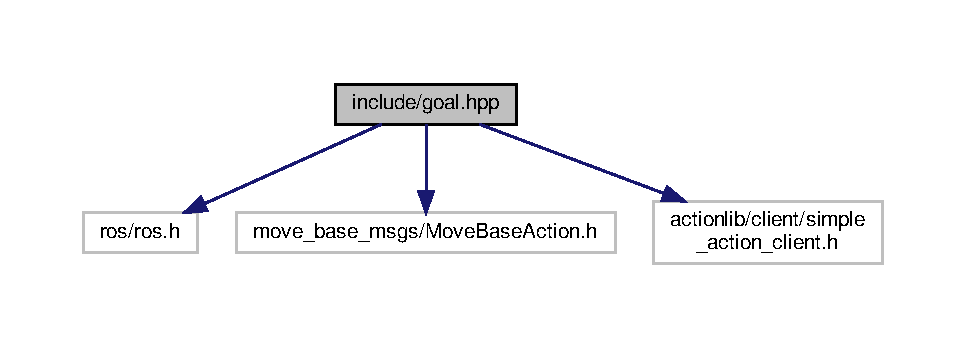
\includegraphics[width=350pt]{goal_8hpp__incl}
\end{center}
\end{figure}
This graph shows which files directly or indirectly include this file\+:
\nopagebreak
\begin{figure}[H]
\begin{center}
\leavevmode
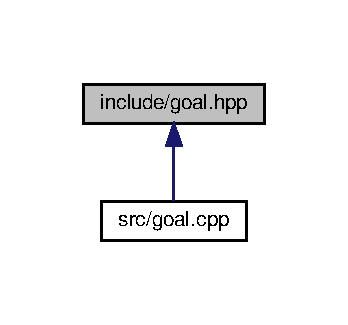
\includegraphics[width=167pt]{goal_8hpp__dep__incl}
\end{center}
\end{figure}
\subsection*{Classes}
\begin{DoxyCompactItemize}
\item 
class \hyperlink{class_goal}{Goal}
\end{DoxyCompactItemize}


\subsection{Detailed Description}
Autonomous Wheelchair. 

\begin{DoxyCopyright}{Copyright}
B\+SD 3-\/\+Clause License 

Copyright © 2020 Raj Shinde, Prasheel Renkuntla, Shubham Sonawane
\end{DoxyCopyright}
\begin{DoxyAuthor}{Author}
Raj Shinde 

Prasheel Renkuntla 

Shubham Sonawane 
\end{DoxyAuthor}
\begin{DoxyDate}{Date}
11/17/2020 
\end{DoxyDate}
\begin{DoxyVersion}{Version}
1.\+0 
\end{DoxyVersion}
\hypertarget{goal_8cpp_Header}{}\subsection{file for sending goals}\label{goal_8cpp_Header}

\hypertarget{goal_8cpp}{}\section{src/goal.cpp File Reference}
\label{goal_8cpp}\index{src/goal.\+cpp@{src/goal.\+cpp}}


Autonomous Wheelchair.  


{\ttfamily \#include \char`\"{}goal.\+hpp\char`\"{}}\newline
Include dependency graph for goal.\+cpp\+:
\nopagebreak
\begin{figure}[H]
\begin{center}
\leavevmode
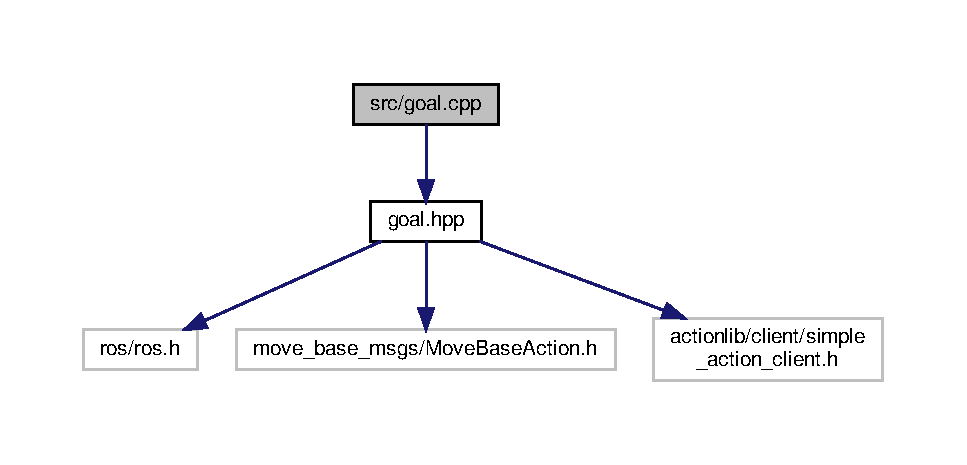
\includegraphics[width=350pt]{goal_8cpp__incl}
\end{center}
\end{figure}
\subsection*{Typedefs}
\begin{DoxyCompactItemize}
\item 
\mbox{\Hypertarget{goal_8cpp_a21e20cc0b6656ae897b3cbb969b93241}\label{goal_8cpp_a21e20cc0b6656ae897b3cbb969b93241}} 
typedef actionlib\+::\+Simple\+Action\+Client$<$ move\+\_\+base\+\_\+msgs\+::\+Move\+Base\+Action $>$ {\bfseries Move\+Base\+Client}
\end{DoxyCompactItemize}
\subsection*{Functions}
\begin{DoxyCompactItemize}
\item 
\mbox{\Hypertarget{goal_8cpp_a3c04138a5bfe5d72780bb7e82a18e627}\label{goal_8cpp_a3c04138a5bfe5d72780bb7e82a18e627}} 
int {\bfseries main} (int argc, char $\ast$$\ast$argv)
\end{DoxyCompactItemize}


\subsection{Detailed Description}
Autonomous Wheelchair. 

\begin{DoxyCopyright}{Copyright}
B\+SD 3-\/\+Clause License 

Copyright © 2020 Raj Shinde, Prasheel Renkuntla, Shubham Sonawane
\end{DoxyCopyright}
\begin{DoxyAuthor}{Author}
Raj Shinde 

Prasheel Renkuntla 

Shubham Sonawane 
\end{DoxyAuthor}
\begin{DoxyDate}{Date}
11/17/2020 
\end{DoxyDate}
\begin{DoxyVersion}{Version}
1.\+0 
\end{DoxyVersion}
\hypertarget{goal_8cpp_Header}{}\subsection{file for sending goals}\label{goal_8cpp_Header}
\begin{DoxyCopyright}{Copyright}
B\+SD 3-\/\+Clause License 

Copyright © 2020 Raj Shinde, Prasheel Renkuntla, Shubham Sonawane
\end{DoxyCopyright}
\begin{DoxyAuthor}{Author}
Raj Shinde 

Prasheel Renkuntla 

Shubham Sonawane 
\end{DoxyAuthor}
\begin{DoxyDate}{Date}
11/17/2020 
\end{DoxyDate}
\begin{DoxyVersion}{Version}
1.\+0 
\end{DoxyVersion}
\hypertarget{goal_8cpp_Implemention}{}\subsection{for providing goals in different rooms}\label{goal_8cpp_Implemention}
\begin{DoxyCopyright}{Copyright}
B\+SD 3-\/\+Clause License 

Copyright © 2020 Raj Shinde, Prasheel Renkuntla, Shubham Sonawane
\end{DoxyCopyright}
\begin{DoxyAuthor}{Author}
Raj Shinde 

Prasheel Renkuntla 

Shubham Sonawane 
\end{DoxyAuthor}
\begin{DoxyDate}{Date}
11/17/2020 
\end{DoxyDate}
\begin{DoxyVersion}{Version}
1.\+0 
\end{DoxyVersion}
\hypertarget{goal_8cpp_Implemention}{}\subsection{for providing goals in different rooms}\label{goal_8cpp_Implemention}

\hypertarget{navigate_robot_8cpp}{}\section{src/navigate\+Robot.cpp File Reference}
\label{navigate_robot_8cpp}\index{src/navigate\+Robot.\+cpp@{src/navigate\+Robot.\+cpp}}


Autonomous Wheelchair.  


{\ttfamily \#include $<$ros/ros.\+h$>$}\newline
{\ttfamily \#include $<$tf/transform\+\_\+listener.\+h$>$}\newline
{\ttfamily \#include $<$geometry\+\_\+msgs/\+Twist.\+h$>$}\newline
{\ttfamily \#include \char`\"{}navigate\+Robot.\+hpp\char`\"{}}\newline
Include dependency graph for navigate\+Robot.\+cpp\+:
\nopagebreak
\begin{figure}[H]
\begin{center}
\leavevmode
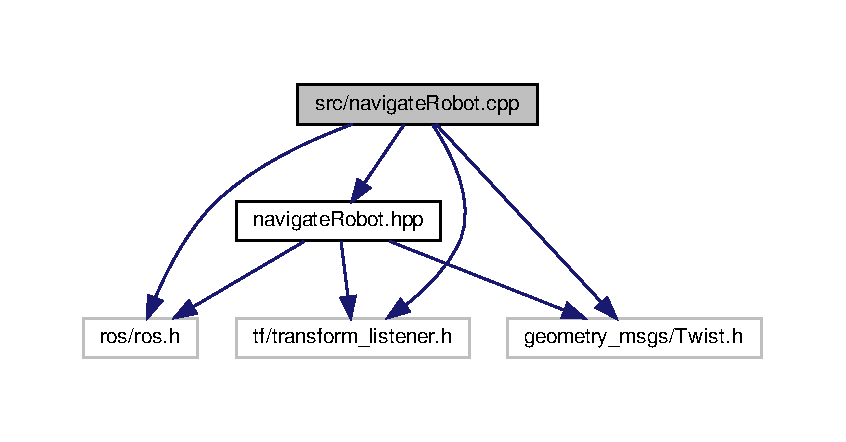
\includegraphics[width=350pt]{navigate_robot_8cpp__incl}
\end{center}
\end{figure}


\subsection{Detailed Description}
Autonomous Wheelchair. 

\begin{DoxyCopyright}{Copyright}
B\+SD 3-\/\+Clause License 

Copyright © 2020 Raj Shinde, Prasheel Renkuntla, Shubham Sonawane
\end{DoxyCopyright}
\begin{DoxyAuthor}{Author}
Raj Shinde 

Prasheel Renkuntla 

Shubham Sonawane 
\end{DoxyAuthor}
\begin{DoxyDate}{Date}
15/11/2020 
\end{DoxyDate}
\begin{DoxyVersion}{Version}
1.\+0 
\end{DoxyVersion}
\hypertarget{path_planner_8cpp_Implementation}{}\subsection{file for navigation of the robot}\label{path_planner_8cpp_Implementation}

\hypertarget{path_planner_8cpp}{}\section{src/path\+Planner.cpp File Reference}
\label{path_planner_8cpp}\index{src/path\+Planner.\+cpp@{src/path\+Planner.\+cpp}}


Autonomous wheelchair.  


{\ttfamily \#include $<$stdio.\+h$>$}\newline
{\ttfamily \#include $<$stdlib.\+h$>$}\newline
{\ttfamily \#include $<$unistd.\+h$>$}\newline
{\ttfamily \#include $<$string.\+h$>$}\newline
{\ttfamily \#include $<$sys/types.\+h$>$}\newline
{\ttfamily \#include $<$sys/socket.\+h$>$}\newline
{\ttfamily \#include $<$netinet/in.\+h$>$}\newline
{\ttfamily \#include $<$netdb.\+h$>$}\newline
{\ttfamily \#include $<$ros/console.\+h$>$}\newline
{\ttfamily \#include $<$pluginlib/class\+\_\+loader.\+h$>$}\newline
{\ttfamily \#include $<$pluginlib/class\+\_\+list\+\_\+macros.\+h$>$}\newline
{\ttfamily \#include $<$set$>$}\newline
{\ttfamily \#include $<$numeric$>$}\newline
{\ttfamily \#include $<$fstream$>$}\newline
{\ttfamily \#include $<$iostream$>$}\newline
{\ttfamily \#include $<$iomanip$>$}\newline
{\ttfamily \#include $<$iterator$>$}\newline
{\ttfamily \#include $<$algorithm$>$}\newline
{\ttfamily \#include $<$string$>$}\newline
{\ttfamily \#include $<$vector$>$}\newline
{\ttfamily \#include $<$map$>$}\newline
{\ttfamily \#include $<$limits$>$}\newline
{\ttfamily \#include \char`\"{}path\+Planner.\+hpp\char`\"{}}\newline
Include dependency graph for path\+Planner.\+cpp\+:
\nopagebreak
\begin{figure}[H]
\begin{center}
\leavevmode
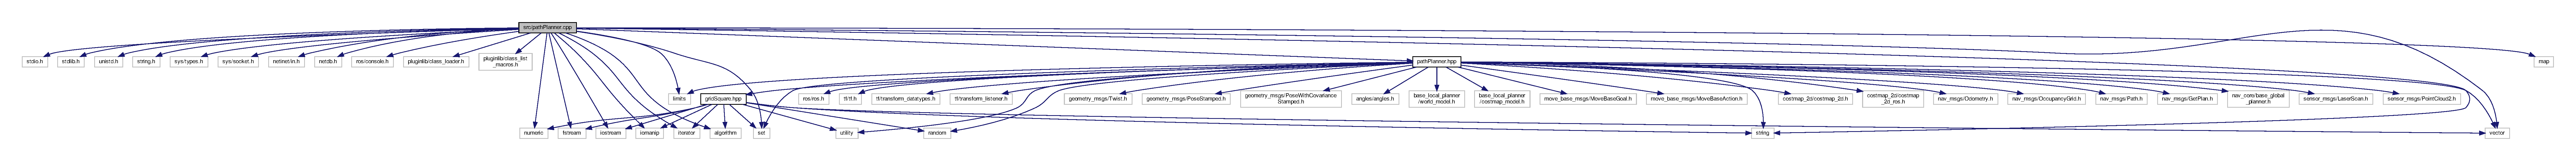
\includegraphics[width=350pt]{path_planner_8cpp__incl}
\end{center}
\end{figure}
\subsection*{Functions}
\begin{DoxyCompactItemize}
\item 
\mbox{\Hypertarget{path_planner_8cpp_a7333a98920b802a9d5d861496d67b1f3}\label{path_planner_8cpp_a7333a98920b802a9d5d861496d67b1f3}} 
bool {\bfseries operator$<$} (\hyperlink{class_grid_square}{Grid\+Square} const \&c1, \hyperlink{class_grid_square}{Grid\+Square} const \&c2)
\end{DoxyCompactItemize}


\subsection{Detailed Description}
Autonomous wheelchair. 

\begin{DoxyCopyright}{Copyright}
B\+SD 3-\/\+Clause License 

Copyright © 2020 Raj Shinde, Prasheel Renkuntla, Shubham Sonawane
\end{DoxyCopyright}
\begin{DoxyAuthor}{Author}
Raj Shinde 

Prasheel Renkuntla 

Shubham Sonawane 
\end{DoxyAuthor}
\begin{DoxyDate}{Date}
12/11/2020 
\end{DoxyDate}
\begin{DoxyVersion}{Version}
1.\+0 
\end{DoxyVersion}
\hypertarget{path_planner_8cpp_Implementation}{}\subsection{file for navigation of the robot}\label{path_planner_8cpp_Implementation}

\hypertarget{test_grid_square_8cpp}{}\section{test/test\+Grid\+Square.cpp File Reference}
\label{test_grid_square_8cpp}\index{test/test\+Grid\+Square.\+cpp@{test/test\+Grid\+Square.\+cpp}}


Autonomous Wheelchair.  


{\ttfamily \#include $<$gtest/gtest.\+h$>$}\newline
{\ttfamily \#include \char`\"{}grid\+Square.\+hpp\char`\"{}}\newline
Include dependency graph for test\+Grid\+Square.\+cpp\+:
\nopagebreak
\begin{figure}[H]
\begin{center}
\leavevmode
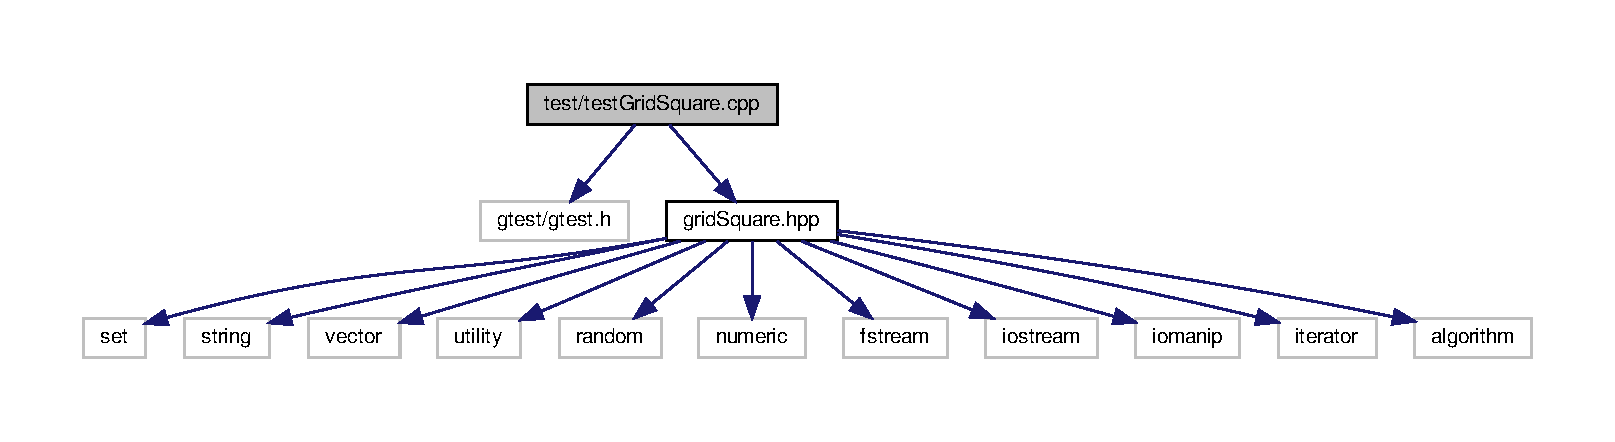
\includegraphics[width=350pt]{test_grid_square_8cpp__incl}
\end{center}
\end{figure}
\subsection*{Functions}
\begin{DoxyCompactItemize}
\item 
\mbox{\Hypertarget{test_grid_square_8cpp_a8642e37efe28c645b3328e697b8687aa}\label{test_grid_square_8cpp_a8642e37efe28c645b3328e697b8687aa}} 
{\bfseries T\+E\+ST} (Test\+Grid\+Square, test\+Get\+Current\+Square)
\item 
\mbox{\Hypertarget{test_grid_square_8cpp_aab22a65713fc4a625bca360127f54b4c}\label{test_grid_square_8cpp_aab22a65713fc4a625bca360127f54b4c}} 
{\bfseries T\+E\+ST} (Test\+Grid\+Square, test\+F\+Cost)
\item 
int \hyperlink{test_grid_square_8cpp_a3c04138a5bfe5d72780bb7e82a18e627}{main} (int argc, char $\ast$$\ast$argv)
\begin{DoxyCompactList}\small\item\em Main Function for running tests of \hyperlink{class_grid_square}{Grid\+Square} Class. \end{DoxyCompactList}\end{DoxyCompactItemize}


\subsection{Detailed Description}
Autonomous Wheelchair. 

\begin{DoxyCopyright}{Copyright}
B\+SD 3-\/\+Clause License 

Copyright © 2020 Raj Shinde, Prasheel Renkuntla, Shubham Sonawane
\end{DoxyCopyright}
\begin{DoxyAuthor}{Author}
Raj Shinde 

Prasheel Renkuntla 

Shubham Sonawane 
\end{DoxyAuthor}
\begin{DoxyDate}{Date}
11/17/2020 
\end{DoxyDate}
\begin{DoxyVersion}{Version}
1.\+0 
\end{DoxyVersion}
\hypertarget{test_navigate_robot_8cpp_To}{}\subsection{test grid squares of the map. for planner}\label{test_navigate_robot_8cpp_To}


\subsection{Function Documentation}
\mbox{\Hypertarget{test_grid_square_8cpp_a3c04138a5bfe5d72780bb7e82a18e627}\label{test_grid_square_8cpp_a3c04138a5bfe5d72780bb7e82a18e627}} 
\index{test\+Grid\+Square.\+cpp@{test\+Grid\+Square.\+cpp}!main@{main}}
\index{main@{main}!test\+Grid\+Square.\+cpp@{test\+Grid\+Square.\+cpp}}
\subsubsection{\texorpdfstring{main()}{main()}}
{\footnotesize\ttfamily int main (\begin{DoxyParamCaption}\item[{int}]{argc,  }\item[{char $\ast$$\ast$}]{argv }\end{DoxyParamCaption})}



Main Function for running tests of \hyperlink{class_grid_square}{Grid\+Square} Class. 


\begin{DoxyParams}{Parameters}
{\em int} & argc, char argv \\
\hline
\end{DoxyParams}
\begin{DoxyReturn}{Returns}
int 
\end{DoxyReturn}

\hypertarget{test_navigate_robot_8cpp}{}\section{test/test\+Navigate\+Robot.cpp File Reference}
\label{test_navigate_robot_8cpp}\index{test/test\+Navigate\+Robot.\+cpp@{test/test\+Navigate\+Robot.\+cpp}}


Autonomous Wheelchair.  


{\ttfamily \#include $<$ros/ros.\+h$>$}\newline
{\ttfamily \#include $<$tf/transform\+\_\+listener.\+h$>$}\newline
{\ttfamily \#include $<$geometry\+\_\+msgs/\+Twist.\+h$>$}\newline
{\ttfamily \#include $<$std\+\_\+msgs/\+Empty.\+h$>$}\newline
{\ttfamily \#include $<$gtest/gtest.\+h$>$}\newline
{\ttfamily \#include \char`\"{}navigate\+Robot.\+hpp\char`\"{}}\newline
Include dependency graph for test\+Navigate\+Robot.\+cpp\+:
\nopagebreak
\begin{figure}[H]
\begin{center}
\leavevmode
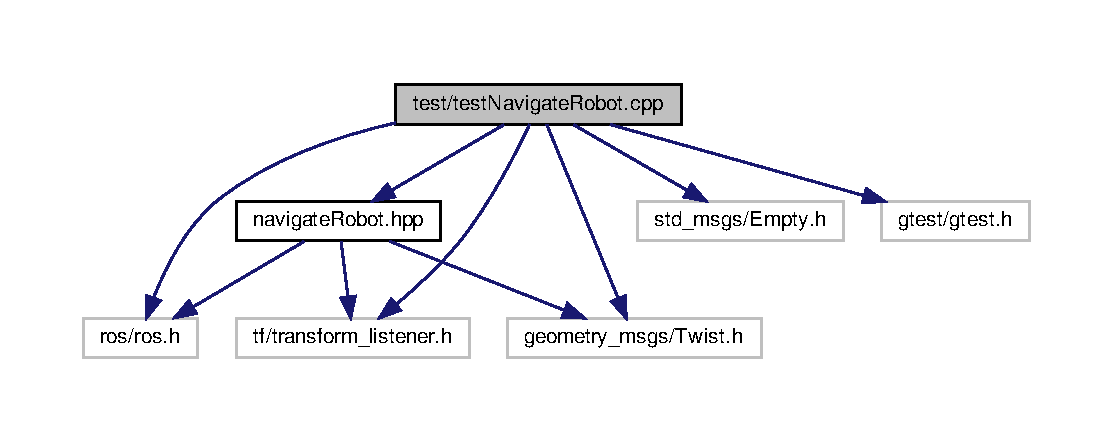
\includegraphics[width=350pt]{test_navigate_robot_8cpp__incl}
\end{center}
\end{figure}
\subsection*{Functions}
\begin{DoxyCompactItemize}
\item 
\mbox{\Hypertarget{test_navigate_robot_8cpp_ab63cc19d361017bcaeafdd6dcaf90c0f}\label{test_navigate_robot_8cpp_ab63cc19d361017bcaeafdd6dcaf90c0f}} 
{\bfseries T\+E\+ST} (Test\+Navigate\+Robot, test\+Twist\+Robot)
\item 
\mbox{\Hypertarget{test_navigate_robot_8cpp_ab9381bbc210f36b78e67f433aa51b662}\label{test_navigate_robot_8cpp_ab9381bbc210f36b78e67f433aa51b662}} 
{\bfseries T\+E\+ST} (Test\+Navigate\+Robot, test\+Start)
\item 
int \hyperlink{test_navigate_robot_8cpp_a3c04138a5bfe5d72780bb7e82a18e627}{main} (int argc, char $\ast$$\ast$argv)
\begin{DoxyCompactList}\small\item\em Main Function for running tests for Navigate Robot Class. \end{DoxyCompactList}\end{DoxyCompactItemize}


\subsection{Detailed Description}
Autonomous Wheelchair. 

\begin{DoxyCopyright}{Copyright}
B\+SD 3-\/\+Clause License 

Copyright © 2019 Raj Shinde, Prasheel Renkuntla, Shubham Sonawane
\end{DoxyCopyright}
\begin{DoxyAuthor}{Author}
Raj Shinde 

Prasheel Renkuntla 

Shubham Sonawane 
\end{DoxyAuthor}
\begin{DoxyDate}{Date}
15/11/2020 
\end{DoxyDate}
\begin{DoxyVersion}{Version}
1.\+0 
\end{DoxyVersion}
\hypertarget{test_navigate_robot_8cpp_To}{}\subsection{test grid squares of the map. for planner}\label{test_navigate_robot_8cpp_To}


\subsection{Function Documentation}
\mbox{\Hypertarget{test_navigate_robot_8cpp_a3c04138a5bfe5d72780bb7e82a18e627}\label{test_navigate_robot_8cpp_a3c04138a5bfe5d72780bb7e82a18e627}} 
\index{test\+Navigate\+Robot.\+cpp@{test\+Navigate\+Robot.\+cpp}!main@{main}}
\index{main@{main}!test\+Navigate\+Robot.\+cpp@{test\+Navigate\+Robot.\+cpp}}
\subsubsection{\texorpdfstring{main()}{main()}}
{\footnotesize\ttfamily int main (\begin{DoxyParamCaption}\item[{int}]{argc,  }\item[{char $\ast$$\ast$}]{argv }\end{DoxyParamCaption})}



Main Function for running tests for Navigate Robot Class. 


\begin{DoxyParams}{Parameters}
{\em int} & argc, char argv \\
\hline
\end{DoxyParams}
\begin{DoxyReturn}{Returns}
int 
\end{DoxyReturn}

%--- End generated contents ---

% Index
\backmatter
\newpage
\phantomsection
\clearemptydoublepage
\addcontentsline{toc}{chapter}{Index}
\printindex

\end{document}
